\chapter{Methods}

In this chapter we will discuss the methods and equipment that were used to engineer the samples and perform the experiments presented in the following chapter. During my Master's course, the main activities that I was undertaking were (in the chronological order):
\begin{itemize}
\item designing chips for investigating Q-factors of superconducting CPW resonators
\item designing chips with cQED systems based on transmons
\item improving experimental setup at RQC (design of PCBs, extending fridge capacity, developing software)
\item studying the Q-factors of resonators made of different superconductors
\item spectroscopy of the cQED samples
\item building a time-domain setup for XY-control and dispersive readout of a single qubit
\item time-resolved measurements
\end{itemize}  

Most of the spectroscopy was done at Institute of Solid State Physics in the Russian Quantum Center (RQC) lab and the time-resolved experiments were performed in the Artificial Quantum Systems Lab at Moscow Institute of Physics and Technology. Therefore, the setups in these two places will be used to illustrate the corresponding type of the experiment. 

First of all, some words about EM-simulations and the process of the chip design will be said, concerning both qubits and resonators. Then, the resonator measurement technique will be shown. Finally, we will turn to the qubit measurements, firstly, showing the spectroscopic part and, secondly, elaborating on the time-resolved techniques.

\section{Engineering of the samples}

\subsection{Designing CPW resonators}

\begin{figure}[t]
\includegraphics[width=\textwidth]{resonators_design_perspective}
\caption{Design perspective for the resonator samples that were studied. All resonators had the center strip width of 7 $\mu$m and the coplanar gaps of 4 $\mu$m. \textbf{(a)} Initial design, 10$\times$5 mm$^2$. Six resonators are located near the feedline, with and without an IDC at the open end (used to couple to the transmons in cQED). The asymmetric contact pad configuration was chosen to be compatible to the PCBs which were available at that moment. Resonant frequencies were non-uniformly distributed from 6 to 8.6 GHz. External quality factors were calculated to be around 6000 based on simulated transmission data. \textbf{(b)} Second version of the design. The main differences are the doubled number of the resonators on the chip (to gather more accurate statistical data) and the $Q_e$ increased up to $10^{5}$ (to facilitate the extraction of the $Q_i$ for the fitting algorithm). The frequencies were uniformly distributed from 6 to 8.2 GHz. Also, a border to simplify cutting the chips out of the waver and an ID-label to help distinguish between the samples were added. \textbf{(c)} Third iteration of the design with 24 resonators. Parameters are the same as for the second version, but the size was increased, and the contact pads adapted to the 10$\times$10 mm$^2$ PCBs.}
\label{fig:resonators_design_perspective}
\end{figure}

The CPW resonators that I wanted to use are the $\lambda/4$-type ones, coupled to the feedline as shunts (notch-type). During the 2 years of my work, I have gone through just three design versions for the samples with almost no change for the geometries of the individual resonators. This is very important: we were studying the influence of the fabrication process on the quality factors, and thus to have consistent results between different samples and to have the right to compare them one with other, at least their in-plane geometries had to be identical. The designs that were used are presented in \autoref{fig:resonators_design_perspective} in the chronological order. 

The first design, despite its simplicity, included a lot of work and formed a foundation for the future developments. It was already extensively simulated, allowed to test experimentally the semi-analytic formula\cite{Sank2014} that estimates the ``claw''-coupler influence on the resonance frequency, to test the simulated coupling Q-factors, etc. However, the main feature behind it, which was at that time a breakthrough for me and our group in Russia, was that no hand-drawing at all had been involved in its creation. In contrast, the layout was fully parametrized and programmed using the macro API of the \textit{LayoutEditor} EDA software. This technique of coding the design, though tedious in the beginning, allows in the long run to make such complex changes to the scheme which otherwise would require redrawing everything from scratch. Moreover, the algorithm, once done correctly and debugged, will make no mistakes which are inevitable when the blueprints are modified by hand. Finally, the basic structures and boolean strategies between layers that were implemented to create that first chip are still being reused and extended by me and other people in the group, which means no extra unnecessary work is done. I would like to thank Jürgen Lisenfeld from Karlsruhe Institute of Technology for showing me this method and saving days of my life from being wasted on redrawing and checking designs for errors after any change.

The  second design was mostly the same as the first one to ensure consistency between the experiments. It was embellished with a border of width equal to the half thickness of the diamond saw blade (50 microns) to facilitate dicing of the wafers and a label with a unique identifier for each sample. The external quality factors were increased up to $\approx 10^{5}$ for the resonators in this design by moving them further away from the feedline. This helps to find the internal Q-factors more accurately since the fitting algorithm, which will be described in more detail in \autoref{sec:circlefit}, finds $Q_e$ and $Q_l$ from the data, and then calculates the remaining factor from these two values (recall equation \eqref{eq:qfactor} from chapter 1). If the internal Q-factor is much higher than the external one, then $Q_e$ and $Q_i$ are nearly the same, and the error for the $Q_i$ may become large. To avoid such situations, $Q_e$ was made comparable to the highest measured $Q_i$. The number of the resonators was increased to 12 to increase the statistical sample and to be more confident in the obtained results.

The third design was filled with 24 resonators to increase the statistical accuracy even more. Otherwise, it was quite the same as the previous one.

\subsection{Simulation of CPW resonator response}

\begin{figure}[t]
\centering
\includegraphics[height=0.4\textheight]{sim_res_S21}\quad \includegraphics[height=0.4\textheight]{res_response}
\caption{Simulated $S_{21}(f)$ (left) and electrical in-plane current density near resonance (right) for an example design. The modelling was done in \textit{Sonnet Suite} 2.5D FEM software designed especially for simulating such planar structures. By fitting the parametrically plotted curve $S_{21}(f)$ in the complex plane, which is ideally a circle, the frequency and the Q-factors of the resonance may be extracted.}
\label{fig:sim_res_s21}
\end{figure}

Having the design, it is possible to directly import it into the EM-simulation software. \textit{Ansoft HFSS} is usually used for full 3-dimensional analysis, though for S-parameter computation a 2.5D-solver \textit{Sonnet Suite} is usually enough. The Sonnet simulation engine \textit{em} models the 2D structure as follows: first, it places it between two dielectric layers of given thickness and relative permittivities $\varepsilon_{1,2}$; then, this 3-layer structure is placed inside a grounded rectangular box made of perfect electric conductor. The sought S-parameters are selected by placing \textit{ports} between the ground and the electrode on which we want to set or measure the voltage. Finally, by solving the Maxwell equations in frequency domain, the voltages across the ports are found. 

Typical results for such simulation cab be observed in \autoref{fig:sim_res_s21}. The complex $S_{21}$ parameter is calculated for the ports at the feedline for each frequency. To find a single resonator response in the vicinity of its resonance frequency, Sonnet adaptive solver usually needs three frequencies at which it performs the full solution. Then it interpolates the S-parameters for the resting points and yields smooth curves which can be fitted to find the properties of the resonator under study. This interpolation is rather accurate, and thus it is practical to put a larger number of points to be interpolated so that extraction of the parameters may be done after a single run without the need of several zoom-in simulations.

Another observation for the Sonnet solver is that it gives a noticeably non-circular but rather flattened elliptical response on the complex plane around the resonant frequency when the loss is introduced into the dielectric layers; it produces a non-ideally circular response when there is no loss at all, too. That means it is not possible to find the internal Q-factor by fitting the simulation data, since it is defined exactly by the area that loses its shape. It is not clear why this is the case, as long as in the experiment the curves show such flattening only when non-linear effects come to play.\cite{astafiev2010}

The EM-simulations are quite heavy when large curved structures are considered. To perform a simulation like one shown in \autoref{fig:sim_res_s21} in an hour, it takes several gigabytes of RAM and two Intel Xeon E5-2670 processors. This computational complexity has led to development of different analytic models for estimating the external Q-factors and coupling capacitances of such structures\cite{martinis2014}; however, these methods are not simple to implement in practice and also are not very accurate. Therefore, in my work the main reference that I used was simulation data.

\subsection{Calculating transmon parameters}

\subsubsection{Capacitances}

For the transmons that were used in the experimental part of this work the only calculated parameters were the island capacitance to the ground and the coupling capacitance between the island and the open end of the resonator. These values were calculated using Sonnet by putting an autogrounded port on the qubit island and a usual port on the resonator central strip. 

\begin{figure}
\centering
\begin{minipage}{0.45\textwidth}
\includegraphics[height=0.4\textheight]{xmon_cap+g}
\end{minipage}\quad
\begin{minipage}{0.45\textwidth}
\includegraphics[height=0.35\textheight]{xmon_cap_mipt_re}

\vspace*{0.5cm}
\end{minipage}
\caption{Capacitances of the transmon island to the ground and between the island and the resonator in dependence on frequency extracted from the admittance parameters $Y_{11}$ and $Y_{21}$ (left) and in-plane current density calculated by Sonnet solver for this structure.}
\label{fig:xmon_cap}
\end{figure}

It is important that Sonnet uses the following formulas to calculate the capacitances (assuming the PI-model) from the Y-matrix:
\begin{itemize}[topsep=0pt, noitemsep]
\item from the reflection admittance $Y_{11}$: $C = -(\omega \mathfrak{Im}[1/Y_{11}])^{-1}$
\item from the transmission admittance $Y_{21}$: $C = (\omega \mathfrak{Im}[1/Y_{21}])^{-1}$
\end{itemize}
This means that if, for example, the connection between two ports is inductive or if a single port is connected to a polygon going into the ground, Sonnet will blindly follow these expressions and show negative capacitances. However, sometimes negative capacitances appear even in a correctly designed simulation after the \textit{de-embedding} process that affects interpolation; thus, only the directly calculated frequencies should be taken into account. Finally, negative capacitances sometimes appear for no clear reason and only can be overcome by changing the design parameters.

In \autoref{fig:xmon_cap} the results obtained from a two-port simulations are presented. The self-capacitance of the transmon's island and the coupling capacitance to the resonator end is calculated in a single run by looking at $Y_{11}$ and  $Y_{21}$. One can notice that their values grow with frequency; Sonnet manual explains this effect by increasing fringing fields between the fingers. However, I couldn't find any rigorous description of this effect and, since the increase is quite small, I don't take it into further calculations.

\subsubsection{Josephson junctions}

To achieve the desired $ge$ transition frequency it is not sufficient to calculate only the capacitance of the transmon's island. Recalling equation \eqref{eq:tr_levels} from Chapter 1, we see that Josephson energy $I_c h/2e$ is no less important. In practice, only the critical current is required for making the design. Usually, the calibration curve which links the oxidation exposure of the JJs with the critical current density $j_c$ is known, so it's sufficient to choose a point with a definite $j_c$ and then just calculate the required area of the junctions.

In drawing the junctions for a Dolan-bridge\cite{dolan1977} mask, two things about the geometry are important:
\begin{itemize}[topsep=0pt, noitemsep]
\item the bridge should be around 100 nm wide and around 200 nm long so that it won't sag 
\item structures near the bridge should not be very large due to the proximity effect of the electron beam
\end{itemize}

The evaporation angle needed for two layers of the junctions to overlap correctly can be found using the following formula:

\[
\zeta = \frac{180}{\pi}\arctan\rbrkt{\frac{W+w}{2H+h}},
\]
where $W$ is the width of the thinnest electrode, $w$ is the width of the bridge, $H$ is the height of the co-polymer (lower layer of the mask, $\approx$ 700 nm) and $H$ is the resist thickness (upper layer, $\approx$100 nm). In our established processes, the evaporation angle was rarely above 15 degrees, and this fact also was putting some constraints on the geometry.


\section{Extraction of resonator parameters from its scattering data}\label{sec:circlefit}

In practice, we never observe ideal circular curve on the complex plane when measuring the resonator response. This is caused by environmental contributions which are inevitably present. Such contributions are phase delay due to the length of the wiring that connects the measuring apparatus to the sample, the ideal 50-Ohm symmetric ports are replaced via wirebods of unknown impedance, the total attenuation and amplification before and after the sample is not known exactly. However, according to a paper by S. Probst et al\cite{probst2015}., these contributions may be estimated and ruled out as individual factors in a common formula. Therefore, the frequency response of a notch-type resonator as the $S_{21}$ parameter can be described with a simple formula:
\begin{equation}
S_{21}^{notch}(f) = \underbrace{ae^{i\alpha}e^{2\pi if\tau}}_\text{wiring and amplification} \underbrace{\left[1-\frac{Q_l/Q_e'}{1+2iQ_l(f/f_r-1)}\right]}_\text{mismatched resonator},
\label{eq:res_S21_probst}
\end{equation} 
where $a$ is the total amplification, $\alpha$ is the constant phase offset, $\tau$ is the time that electromagnetic wave needs to traverse the connecting cables (also called electrical or phase delay, approximately equal to 50 ns for a typical dilution fridge setup), $Q_l$ is the loaded Q-factor and $f_r$ is the resonance frequency. Finally, $Q_e'$ is the complex external quality factor. It appears to be complex in the observed $S_{21}(f)$ curve due to the impedance mismatch between the resonator ports\cite{Khalil2012} or due to the standing waves between the wirebonds\cite{Deng2013} (these explanations come from two different models, but the second model is more general). It was also demonstrated that internal quality factor can be extracted from $Q_e'$ and $Q_l$ as follows (\textit{diameter correction method, DCM}):
\[
Q_{i, \text{DCM}}^{-1} = Q_l^{-1} - \mathfrak{Re}[Q'_e]^{-1} .
\]
To sum up, using the formula \eqref{eq:res_S21_probst} to fit the experimental data, we extract all interesting parameters of the resonator. The fitting and the extraction procedure was also conveniently implemented by the author of the paper in a tool called \textit{circlefit} (it is open source and can be found on GitHub \href{https://github.com/sebastianprobst/resonator_tools/tree/master/resonator_tools}{\footnotesize{\faExternalLink}}).


\section{Experimental techniques}

In this section we will discuss hardware and methods that have been used in this work. However, since such discussions are very common in our domain and can be easily found elsewhere, only selected topics will be listed here. 

\subsection{Fridge, wiring and attenuation}

Experiments with superconducting structures working in the quantum regime require cooling of the samples down to the temperatures which ensure low populations of their excited states. Since Josephson junctions of our samples are made of Aluminium, which has a superconducting gap of 80 GHz, and since the microwave equipment (such as low-noise amplifiers) that works under $\approx$15 GHz is cheap, the usual transition frequencies between the ground and the excited states in superconducting qubits are usually close to 10 GHz. This is the reason why the dilution fridges with base temperatures from 10 to 40 mK are used everywhere in the world. I have been working with BlueFors LD250 fridges during writing this thesis.

In practice, the chip with the qubits should not only be cooled down but also connected to the measurement apparatus. It is important that the cables do not bring additional thermal noise to the sample, so they are equipped with microwave attenuators. Usually, the fridge has several stages which are sustained at different temperatures; the lower the stage, the lower the temperature (see \autoref{fig:cryo_wiring}). In most cases, the sample is installed at the lowest stage. Therefore, to remove additional thermal noise near the sample and, at the same time, to diffuse heat uniformly, the microwave attenuators with certain attenuation factors are installed at each stage. To find exactly the optimal factor at each stage, we can approximate the attenuator with a $Z_0=$50 Ohm resistance and then use the formula for the power spectral density (PSD) of its voltage noise (Johnson-Nyquist formula):
\begin{equation}
S^i(f, T) = \frac{2 Z_0 h f}{e^{h f/k_b T}-1},
\label{eq:JN_eq}
\end{equation}
where suffix $i$ stands for ``internal''. The attenuator at stage $T_n$ accepts temperature noise from the stage above which is at $T_{n-1}$, and the residual noise from all stages above. Ideally, when there is no input from hotter stages, this attenuator itself (still, approximated with a resistance) will produce internal noise with PSD $S_n^i(f) = S^i(f, T_n)$. This is the lowest achievable PSD at that stage, so we need to bring the full PSD
\begin{equation}
S_n(f) = S_n^i(f) + \alpha_n S_{n-1}(f)
\label{eq:full_th_PSD}
\end{equation}
close to this value, making $\alpha_n S_{n-1}\ll S^i_{n}$, where $\alpha_n$ is the attenuation constant  
at stage $n$ in absolute units.

\begin{table}
\centering
\begin{tabular}{l|c|c|c|c|c|c}
\hline
Temperature [K] & 43 & 3.3 & 1 &0.1 & 0.02 & $T_{eff}$ \\
\hline
$\alpha_n$,  ideal [dB] & -8 & -11 & -6 & -17 & -50 &23 mK \\
$\alpha_n$, practical [dB] & 0 & -10 & -10 & -20 & -20 & 47 mK\\
\hline
\end{tabular}

\caption{Configurations to achieve various effective temperatures at the lowest stage. Calculated using the full equation \eqref{eq:full_th_PSD} and solving \eqref{eq:JN_eq} for $T_{eff}$. It can be seen that it is impractical to try to match the temperature of the lowest stage since in the quantum limit the PSD defined by \eqref{eq:JN_eq} decreases exponentially with temperature and requires us to put a lot of attenuation at the lowest stage.}
\label{tab:attenuation}
\end{table}

Mathematically this will look as follows: $\alpha \ll {S^i_n}/{S_{n-1}}$. We could say that $\alpha$ should be, for instance, 1/10th of ${S^i_n}/{S_{n-1}}$ to keep only two subsequent stages in our calculation and forget about the others; however, it can be shown that the noise temperature at the lowest stage at mK and few GHz will not be significantly affected even if $\alpha$ is chosen to be equal to 1. Thus, the final expression goes below:
\[
 \alpha \approx  {S^i_n}/{S^i_{n-1}} =  \frac{e^{hf/k_b T_{n-1}} -1}{e^{hf/k_b T_n}-1}.
\]

If the temperatures are high, so that $k_b T \gg hf$ at interesting frequencies (near 6 GHz this will occur if T $\gg$ 200-300 mK), then the formula for the attenuation becomes
$$
\alpha \approx T_n/T_{n-1}.
$$
For example, let's assume $T_n = T_1 = 50K, T_{n-1} = T_0 = 300K$. In this case $\alpha = 1/6 \approx 0.1 = -10$ dB. 

In practice, however, it is possible to sacrifice the uniformity of the thermal dissipation across the stages in favour of reduced overall attenuation. In \autoref{fig:cryo_wiring} a schematic of our fridge with a typical configuration of the wiring inside it is presented. The configuration of the attenuators was chosen to be as depicted in \autoref{tab:attenuation}, practical. It gives a 47 mK effective noise at the lowest stage instead of its own temperature of 20 mK; however, 20 mK is actually a much smaller temperature than we need because at 6 GHz and 47 mK the excited state already is only populated with probability of $\approx$0.2\% (compare to the less than $10^{-6}$ probability at 20 mK). In addition, matching the base temperature requires us to put a huge amount of attenuation at the low-temperature stages, i.e. 100 mK and 20 mK stages (see \autoref{tab:attenuation}, ideal configuration); this is totally impractical as long as it is impossible to generate signals strong enough to pass through this attenuation to the sample and still have any effect on it. So this is why we do not put any attenuation at the highest stage and reduce the attenuation at the lowest stage compared to the calculated ideal configuration.

The output line cannot be attenuated to isolate the environment since the already weak signal going from the sample will be completely lost. Therefore, we use two cryogenic circulators with 50-Ohm stubs on the 3\textsuperscript{d} ports or isolators; they each provide a 20 dB directional attenuation for the incoming noise and no loss for the signal. The HEMT amplifier also does not let the noise go down from the 43K and 300K levels.

Additionally to the noise suppression, the attenuators are very useful in minimizing heat conduction through the coaxial cables. They are usually made of stainless steel with conducts heat badly, and thus it was possible to extend the fridge wiring 3 lines made of cables having copper ground shield without any noticeable increase in base temperature.

\begin{figure}
\centering
\includegraphics[width=\textwidth]{setup}
\caption{A scheme of a typical setup for spectroscopic measurements including the basic spectroscopic microwave equipment and wiring inside the fridge. Here 4 coaxial microwave lines are used (3 input and 1 output) with 60 dB of attenuation and 1 coaxial DC-line to tune the qubit with an on-chip flux loop equipped with 20 dB of attenuation and a 500 MHz low-pass filter. Three sample holders are installed, one in a cryoperm shield with a bias coil around it (for resonator and qubit measurements) and the other two unshielded having no coil (mostly for resonator measurements).}
\label{fig:cryo_wiring}
\end{figure}

\begin{figure}[t]
\centering
\includegraphics[width=\textwidth]{BF_for_albmstu1}
\caption{Example configuration of the 20 mK stage of the BF LD 250 fridge in the RQC lab at ISSP with three samples installed (with false colors added). \textbf{(a)} Front-bottom view of the stage. Cyan color highlights the cylindric cryoperm shield inside which the sample holder resides. \textbf{(b)} Back view, violet color shows the circulators with a thick copper wire wrapped around them for thermalization. \textbf{(c)} Front-top view, where the 2-channel  microwave switch is shown (magenta) and the hybrid coupler (blue, left in true color) used to measure several samples using only one low-noise HEMT amplifier. \textbf{(d)} Side view, the two unshielded sample holders similar to the one concealed under the shield from (a) are shown in yellow.}
\label{fig:configuratio_photo}
\end{figure}

\subsection{Spectroscopic measurements}

Spectroscopic measurements are an indispensable tool in resonator and qubit characterization. Below we will discuss how standard spectroscopic experiments with resonators and cQED-systems is performed.

\subsubsection{Single-tone spectroscopy}

This type of experiment in our domain is performed using a heterodyne-detection device called a Vector Network Analyzer (VNA). This device can  generate a tone on one port and than compare it with the signal arriving on the other port (or even on the same one), experimentally acquiring this way the scattering parameters or the S-matrix of the device under test. It can also sweep the frequency of the tone, making it possible to find $S(\omega)$ for the sample. Therefore, it is a very useful tool to study, e.g., resonator response in the frequency domain.

To perform a measurement of a resonator  chip to study quality factors, the following steps should be followed:
\begin{itemize}[topsep=5pt, itemsep=5pt]
\item Scan through a wide range of frequencies at high power of around -10 dBm, high bandwidth of 5 kHz and no averaging (this should work with 60 dB of attenuation as discussed  above), look at the amplitude and the unwrapped phase for any sharp peaks or dips. The phase should be straightened with the correct electrical delay set up in the VNA (around 50 ns for a standard experiment). Usually, the resonances are grouped and linearly distributed in frequency by design, so it is relatively easy to find them all.
\item Zoom in at each resonance and perform a scan at each power from -60 dBm (usually this means -140 dBm at the chip, which corresponds to a single-photon level in most cases) up to 0 dBm with some number of steps; you may want to decrease the averages count $N$at each subsequent power with a following formula:
\[
N(P) = N_{start} 10^{-\frac{P-P_{start}}{P_{end}-P_{start}} \log N_{start} }
\]
with $N_{start}$ equal to $\approx 500$. This will increase the speed of the experiment exponentially while maintaining the same accuracy since the SNR decreases exponentially when power is increased linearly in dBm. $N_{start}$ should be large enough so that the exponent has some space to decay in discrete space.
\end{itemize}

When the qubit samples are studied, single-tone spectroscopy will only reveal something beyond just resonances if the magnetic field around the sample is varied and the qubits can thus be tuned into resonance with their resonators; then the notorious anticrossing will be observed.  

\subsubsection{Two-tone spectroscopy}
\label{sec:2tone}

This type of measurement is conducted with an additional microwave tone from the microwave source, which induces the transitions from the ground state of the system to its higher levels, and then transition frequencies from there are being probed by the VNA. Practically this is realized by setting the VNA to measure a single point at the shifted resonator  frequency $\omega_r + \chi_0$ (see \autoref{fig:diagram}). This results in a low transmission in case of a notch type resonator. Then the qubit is biased, and the frequency on the $\mu$-wave source is swept through some values at each given bias. When the frequency of the latter coincides with some allowed transition frequency of the system at given bias, the system leaves its ground state, and the VNA is not probing a correct transition frequency any more. For example, if second tone has induced the qubit's $ge$ transition, the correct resonator frequency would be $\omega_r + \chi_1$ and the lowest transmission would be observed there (see \autoref{fig:diagram} again). Thus, at $\omega_r + \chi_0$ the transmission would become higher than it was when the second tone missed the $ge$ transition. 

In reality, the situation is a bit more complicated as long as constant microwave tone induces damped Rabi oscillations between levels if it is resonant with the corresponding transition, and in the steady state the VNA will be probing transitions from an incoherent mixture of states (i.e. $\hat \rho = \frac{1}{2} [\ket{0, g}\bra{0,g} + \ket{0, e}\bra{0,e}]$) which depends on the drive strength; however, the transmission still ends up being higher when the second tone induces transitions from ground state. All said above can be applied also to the transmission phase, however the phase at resonance will become either higher of lower depending on the direction of the resonance shift as long as the phase behaves linearly around the resonance. It is thus much more sensitive when the width of the resonance peak is larger than the dispersive shift. 

It is possible to easily extract the linewidth of the qubit which was described in Section \ref{subsec:linewidth} if the resonator linewidth is larger than the dispersive shift. This can be done by setting the VNA frequency to the point of smallest transmission and studying the phase data. The phase will be a linear function of the frequency near this point, and the frequency, in its turn, will be a linear function of the population of the excited state. This means that the width at the half maximum of the 2-tone peak will be same as the width of the peak of the population. If, in contrast, the resonator linewidth is smaller than the dispersive shift, it would be necessary to extract the frequency of the resonator for each point and then plot it against the 2$^{\text{nd}}$ tone frequency to preserve the linearity and measure the linewidth correctly.

This method works well in the dispersive limit when the qubit-resonator detuning $\Delta_\omega = \omega_r - \omega_{ge}$ is large compared to the coupling strength $g$.

The second tone can be applied to the sample either via the same line that is used for the resonator excitation or with an additional line connected to a microwave antenna located on the chip or near it. In the first case, the driving power which is seen by the qubit will depend on the resonator-qubit detuning; this drawback is compensated by a significant reduction in the number of excitation lines, especially when there are several cQED systems attached to the same feedline (technique also known as \textit{frequency-multiplexed readout}). In such configuration, several qubits and resonators can be controlled via just a single line.

\subsubsection{Power-scanning experiments}

To calibrate the qubit driving power and the photon number in the resonator, two experiments based on the two-tone spectroscopy are used\cite{schuster2005}. 

First one consists of sweeping the excitation frequency and the excitation power and allows us to directly see the linewidth of the $ge$ transition (recall Section \ref{subsec:linewidth}). This result is very useful since it allows to infer the Rabi frequency of the qubit which would be observed in the time-resolved experiment, and, if this frequency is found to be too low or too high, the attenuation in the line can be corrected beforehand.

Second one is called AC-Stark spectroscopy and uses the fact that the qubit frequency is dependent on the photon number in the resonator. In the dispersive limit, the cQED Hamiltonian will look as follows:
\[
\mathcal{\hat H} = \hbar\omega_r \hat a^\dag\hat a + \frac{1}{2}\hbar(\omega_q+\frac{g^2}{\Delta_\omega}+2\frac{g^2}{\Delta_\omega}\hat a^\dag\hat a)\hat\sigma_z.
\]
From this expression we can see that the qubit now has an effective frequency proportional to the photon number in the resonator. Due to the photon shot noise in the coherent state of the resonator driven by a classical field, the qubit frequency does not actually have a well-defined value but rather constantly fluctuates which in experiment is observed either as a broadened spectral line or as a distinct set of lines each corresponding to some discrete number of photons in the coherent state and having the amplitude proportional to the probability of this number\cite{schuster2007}.

\subsection{Time-resolved measurements}

In this Section we will discuss experiments which require creating and detecting pulses on a time scale of a few nanoseconds. We will also elaborate on the methods that were used to conduct them, including demonstrating the experimental setup and mentioning some caveats and techniques to improve the results.

\subsubsection{Basic experiments: Rabi, T1, Ramsey, Hahn echo}

First of all, we will describe briefly what usually we want to find about the systems that we are studying. The most common and well-known characteristics of qubits are their relaxation rate, $\gamma = 1/T_1$ ($T_1$ is thus called \textit{relaxation time}) and the total dephasing rate $\gamma_\phi^* = \gamma/2 +\gamma_\phi,\ \gamma_\phi$ is the pure dephasing rate (not caused by relaxation). In the experiment, we also need to know the frequency of the Rabi oscillations $\Omega_R$ to be able to generate pulses which perform correct rotations of the qubit state.

In \autoref{fig:tr_exps} four basic experimental sequences that allow extraction of the parameters mentioned above are presented. All these experiments are done by varying the time $\Delta t$ and ultimately produce data curves which then can be fitted with expressions expected from theory; this allows very accurate estimation of the qubit parameters that enter these expressions.

\begin{figure}
\centering
(a)\includegraphics[width=0.4\textwidth]{rabi}\quad (b)\includegraphics[width=.4\textwidth]{decay}

\vspace{0.5cm}
(c)\includegraphics[width=0.4\textwidth]{ramsey}\quad (d)\includegraphics[width=.4\textwidth]{hahn_echo}
\caption{Basic experiments to find out the properties of a superconducting qubit. Blue lines depict a single qubit quadrature, and the green lines the resonator tone (before upconversion, resonator tone is homodyne).\textbf{(a)} Rabi oscillations. Excitation frequency $\omega$ should be $\approx \omega_{ge}$. Allows to find $ \omega_{ge}$, $ T_1$,  $\ket{e}$ approximately; $T_R$, $\Omega_R \Rightarrow (\pi)^x, (\pi/2)^x$ precisely. \textbf{(b)} Relaxation. $\omega\approx\omega_{ge}$. Allows to find $T_1$ precisely. \textbf{(c)} Ramsey oscillations.  $\omega = \omega_{ge}\pm\Delta\omega$. Allows to find $\omega_{ge}$, $T_2^*$ precisely. \textbf{(d)} Hahn echo. $\omega = \omega_{ge}$. Allows to find $T_{2E}$ precisely.}
\label{fig:tr_exps}
\end{figure}

The qubit is controlled with microwave pulses, as described in \autoref{sec:dynamics}. In the Rabi oscillations experiment, the length of a resonant or a nearly-resonant pulse is varied. After its end, the readout occurs. After averaging the values of the complex S-parameter for each excitation duration, we obtain the probability of the qubit to be in the excited state since

\[
S_{measured}(t) = S_{\ket{g}}|\braket{g}{\psi(t)}|^2 + S_{\ket{e}}|\braket{e}{\psi(t)}|^2.
\]

This is an idealized expression, though, as the qubit is still decaying during the readout, and this means that $S_{measured}$ will be different. However, this effect for some reason does not significantly bias the resulting probabilities (this could be calculated from the master equation).

After the Rabi oscillations experiment has been performed, incoherent decay, Ramsey oscillations and Hahn echo can be done. They use $\left(\frac{\pi}{2}\right)^x$- and $(\pi)^x$-pulses in the way that can be seen in \autoref{fig:tr_exps}. For these experiments is crucial that all the pulses are chopped out of the same continuous carrier wave. This is very important when up-conversion is used, as will be seen below.

\subsubsection{Pulse generation and acquisition techniques}

\begin{figure}
\centering
\large (a)\includegraphics[height=0.2\textheight]{db_mixer}\quad (b)\includegraphics[height=0.2\textheight]{iq_mixer}
\caption{Non-linear elements used to obtain modulated of frequency-converted signals in microwave domain. \textbf{(a)} Double-balanced mixer. Has three ports: local oscillator (LO, for UHF input), intermediate frequency (IF, for HF input/output) and radio frequency (RF, for UHF input/output). \textbf{(b)} IQ-mixer. Consists of two standard mixers (symbolized as $\otimes$ blocks), a 90$^\circ$ hybrid coupler and a power divider. Has four ports: in-phase and quadrature (I an Q) IF-ports, RF and LO ports.}
\label{fig:mixers}
\end{figure}

To create and analyse the pulses in the microwave band, a very popular technique called up- and down-conversion is used.  It exploits a non-linear element to combine signals of high frequencies (HF, usually below 500 MHz) with signals of microwave frequencies (ultra-high frequencies, UHF, above 5 GHz) to obtain a modulated signal with an UHF carrier and an HF modulation. This is a simplest way to generate microwave signals with complex (but still not UHF) modulation because otherwise one would need a digital-to-analog converter (DAC) which would work at several GHz to directly synthesize the necessary signal (such devices are much more expensive and actually are overfulfilling our requirements). We also only need to modulate our pulses at HF, and for this purpose we are using \textit{microwave mixers} as non-linear elements. Two types of such devices are show schematically in \autoref{fig:mixers}. We combine continuous UHF waves from our microwave generators with HF signals from our DACs or, in contrast, analog-to-digital converters (ADCs) when detection is considered. 

Both up- and down- conversion come in several different types. Below the notation from the \autoref{fig:mixers} will be used to specify the voltages at the mixers' ports:
\begin{itemize}[topsep=5pt, itemsep=5pt]
\item Homodyne conversion. It involves mixing UHF carrier signal with another signal that is not sinusoidal and which consequently produces an output pulse with same frequency as the carrier wave and the amplitude modulation governed by the second signal. Mathematically, this looks as follows:
\[
V_{RF}(t) = V_{IF}(t) V_{LO} \cos(\omega_{LO} t + \phi) + I_{LO, RF}V_{LO} \cos(\omega_{LO} t + \phi),
\]
where $I_{LO, RF}$ is the isolation between the UHF-carrier input and output ports of the mixer. Similarly, if an incoming UHF pulse is mixed with an UHF continuous wave, it will be demodulated, and a non-sinusoidal signal capturing the envelope of the pulse will come out of IF port of the mixer. 

\item Heterodyne conversion. Carrier signal is the same, and the HF signal is now an amplitude-modulated sine wave of some frequency $f_{IF}$ much lower than the carrier frequency $f_{LO}$. In this case, at the output of the mixer will be the signal containing $f_{LO} \pm f_{IF}$ frequencies called \textit{sidebands} besides the input ones that leak through. Waves at those frequencies will be modulated in the same way as the HF signal:
\[
V_{RF}(t) = V_{IF}(t) V_{LO}\cos(\omega_{IF}t+\phi_{IF}) \cos(\omega_{LO} t + \phi) + I_{LO, RF} V_{LO} \cos(\omega_{LO} t + \phi).
\]
As can be seen, the first term gives $f_{LO} \pm f_{IF}$ frequencies after a trigonometric expansion. Notably, at this point a simple way to control the phases of each sideband signal appears: they are just $\phi\pm\phi_{IF}$, respectively, for the upper/lower one. Since we digitally synthesize the signal $V_{IF}(t)\cos(\omega_{IF}t+\phi_{IF})$, it is easy to make it have any phase we want. Since UHF signal is generated by precision microwave equipment and its phase is constant in time, we then can control the phase of the output signal completely. Down-conversion here occurs in the same manner, and the output HF signals can be digitized using a fast enough ADC to extract their envelope and phase. 

\item Single-sideband suppressed carrier (SSBSC) heterodyne conversion. The same carrier signal is now split via a hybrid coupler into two parts equal in amplitude but having a phase difference of 90$^\circ$. These parts are then mixed with corresponding HF signals, and the outputs are finally combined back again. This is the principle of an IQ-mixer (see \autoref{fig:mixers}). If the HF signals in their turn have 90$^\circ$ difference in phase and equal amplitudes and frequencies, then one of the sidebands will disappear, and the other one will double it's amplitude. It can be easily shown mathematically (omitting the trigonometric expansions):
\[
\begin{aligned}
V_I(t) &= V_{IF}\sin(\omega_{IF} t+ \phi_{IF})\\
V_Q(t) &= V_{IF}\cos(\omega_{IF} t+ \phi_{IF})\\
V_{RF}(t) &= V_{LO} [V_I(t)\cos(\omega_{LO}t)+V_Q(t)\sin(\omega_{LO}t)]  \\
&= V_{LO} V_{IF} \cos(\omega_{IF}t+\phi_{IF} )
\end{aligned}
\]
\end{itemize}
%
\chapter{Experimental results}

\section{Proof-of-concept design}

\subsection{Geometry and parameters}

The first sample that was measured was created from a proof-of-concept design, which was aimed at testing general properties of the simplest Xmon-based cQED systems. The easiest way to gain insight about the structure of the sample is to look at \autoref{fig:first_chip_design_full} where some of the main parts of its design are shown. The chip is 8 mm long and 4 mm wide and consists basically of six isolated qubit-resonator systems. 

All of the resonators were $\lambda/4$ with frequencies designed to be $6, 6.5, 6.9,7,7.1,8$ GHz for devices I-VI, respectively. Their coplanar parameters are $7\,\mu$m for the central wire width and $4\,\mu$m for the gaps.

The qubits were designed to be identical, with $C_\Sigma \approx 80$ fF and $I_{C, \Sigma} = 60$ nA, giving the $\omega_{01}/2\pi \approx 7$ GHz at their flux sweet-spot ($\Phi_{ext}=0$) and anharmonicity of approximately $-230$ MHz.

Two test structures at the sides of the chip were also included to allow direct DC measurement of the SQUIDs created during the shadow evaporation.

\subsection{Purposes and implementation}

The main targets for the chip were:
\begin{enumerate}[label=(\alph*), leftmargin=1.5cm]
\itemsep0pt
 \item to check the measurement setup
 \item to check the calculations for the frequencies and the coupling strengths
 \item to roughly check the coherence of Xmons
 \item to estimate the reproducibility of the junctions 
 \item to observe the AC-Stark shift 
 \item to observe high-power multiphoton transitions and sidebands
 \item to check for the interesting effects caused by different resonator detunings at sweet-spot  
\end{enumerate}

\begin{figure}[h!]
\centering
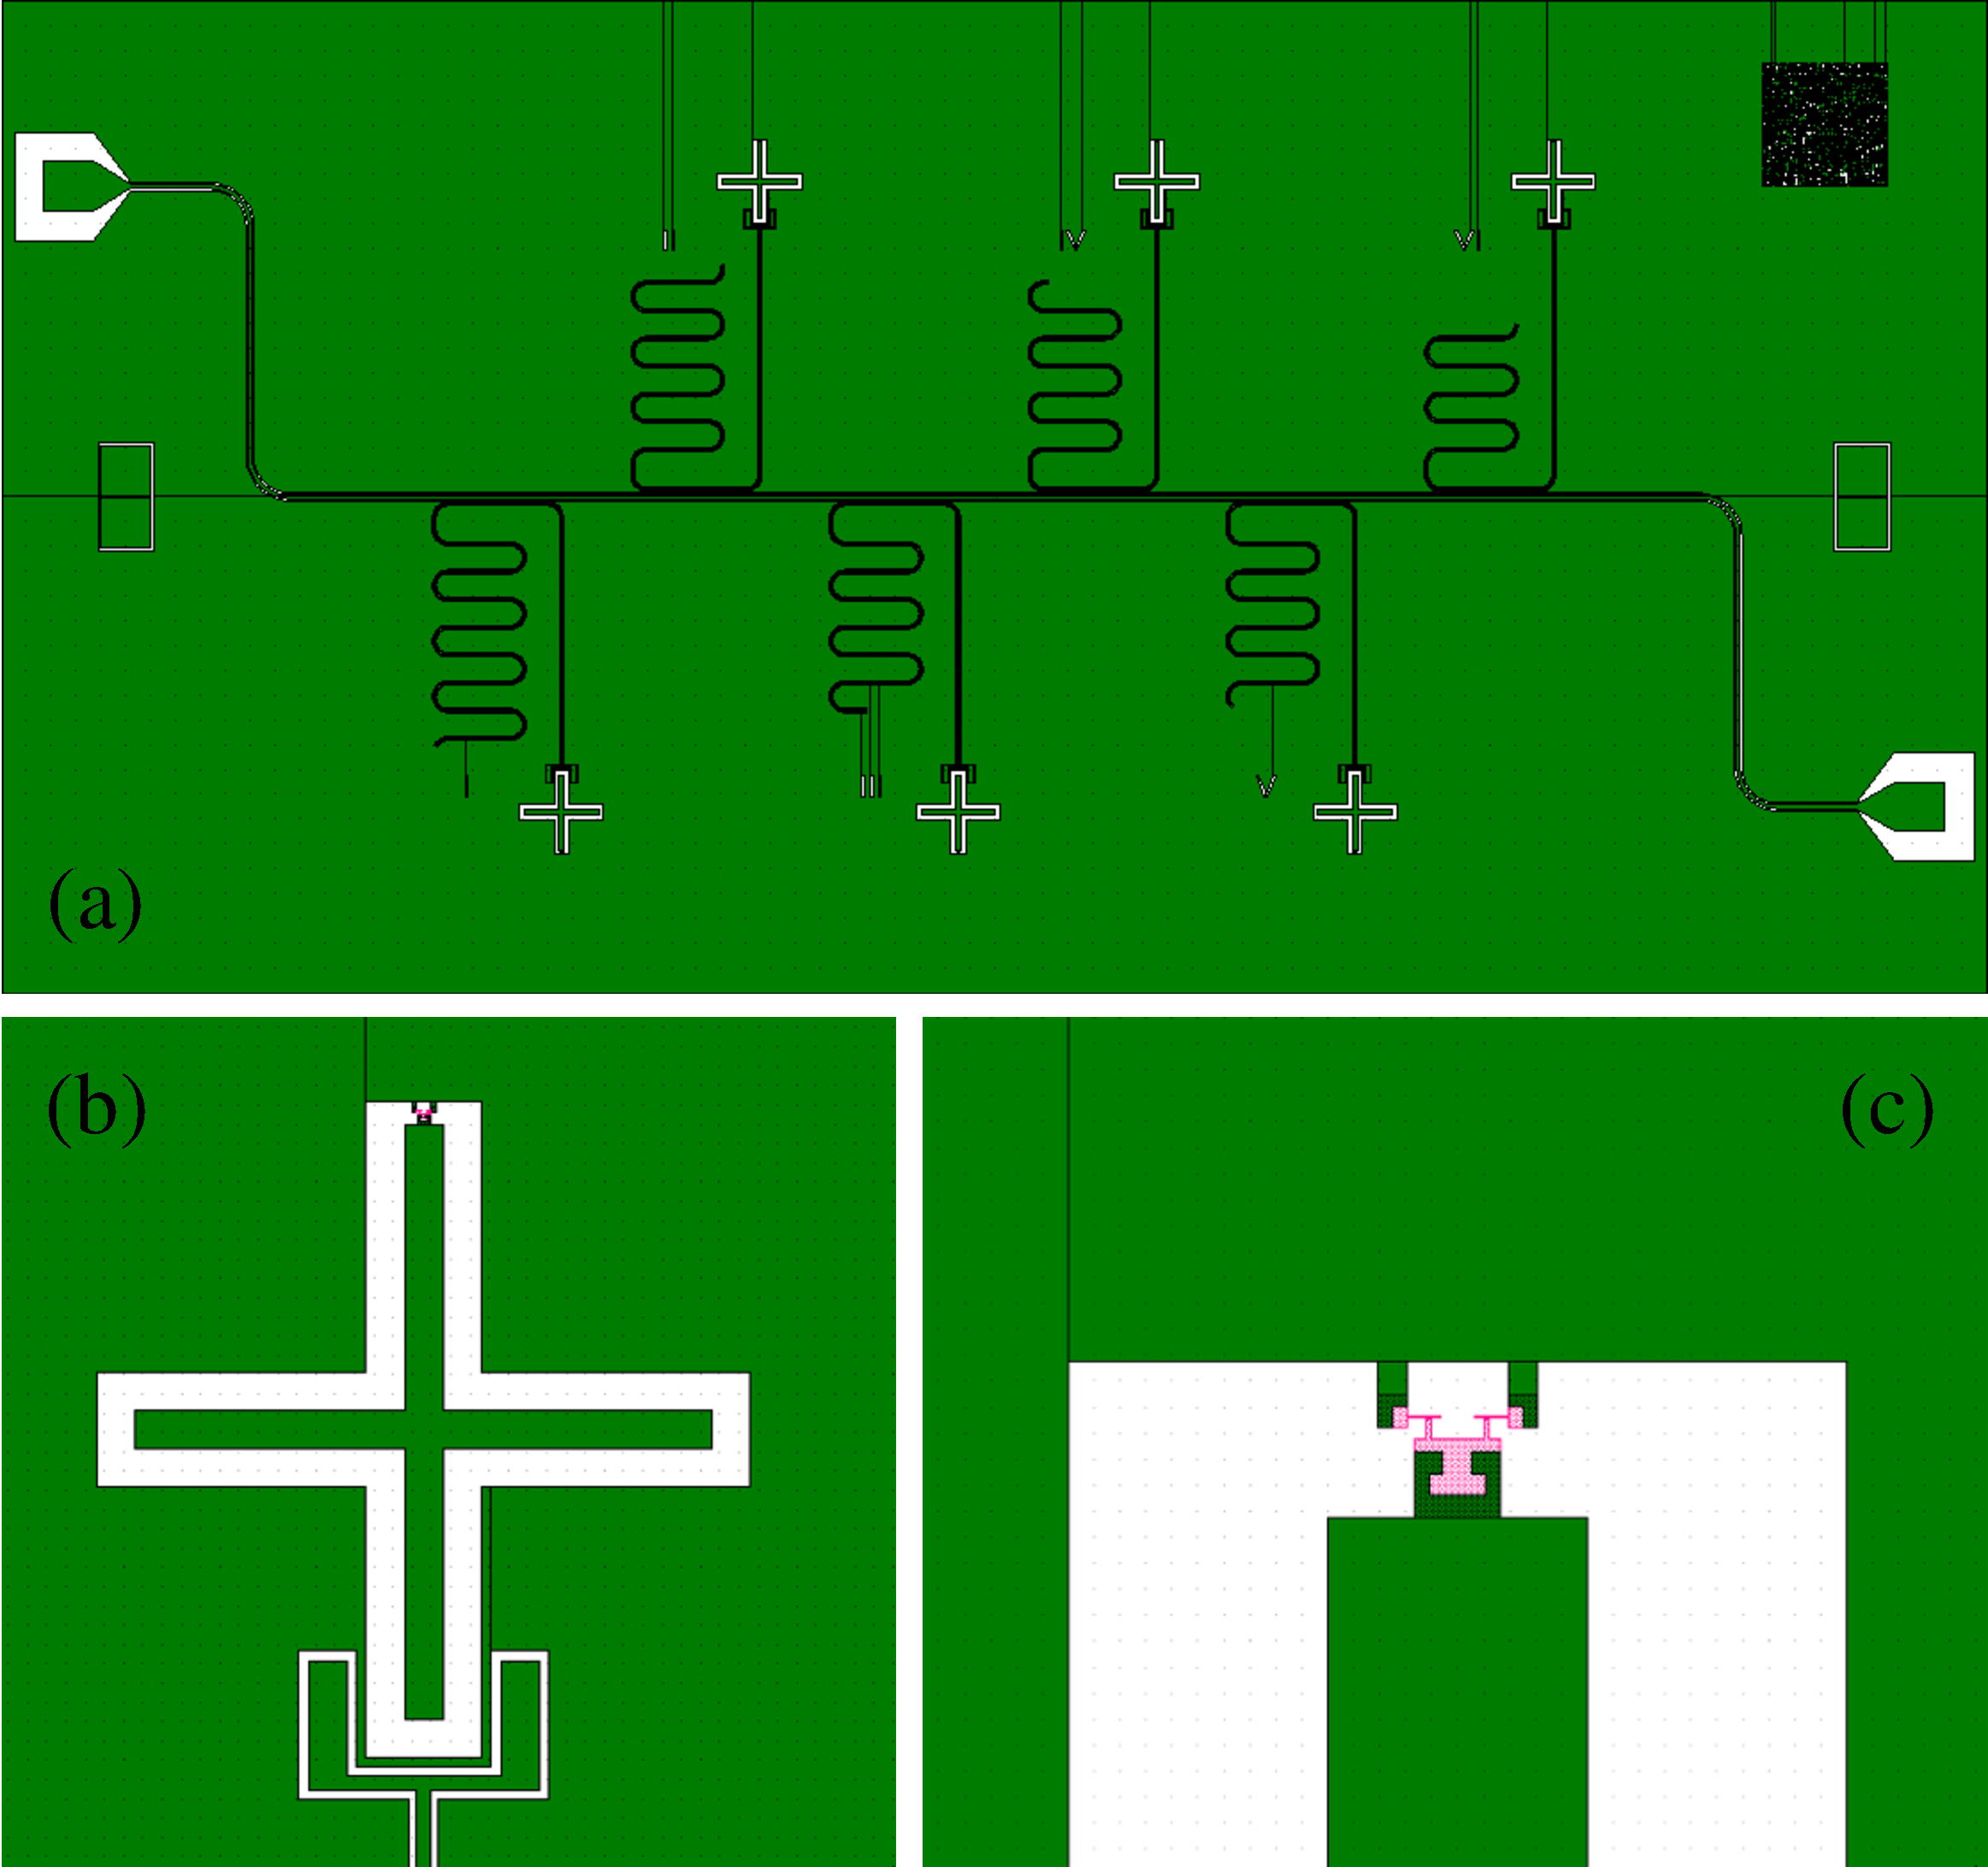
\includegraphics[width=0.9\textwidth]{chip_design_full}
\caption{\textbf{(a)} Large-scale image of the design used for the proof-of-concept sample. The chip (8x4 mm) consists of six $\lambda/4$ CPW resonators coupled capacitively to the feedline each with an Xmon qubit at the open end. \textbf{(b)} Zoomed area around one of the qubits, showing its cross-shaped capacitor and the ``claw'' coupler of its resonator. \textbf{(c)} Zoom around one of the qubits' SQUIDs. Pink areas denote the e-beam mask that was used for shadow evaporation.}
\label{fig:first_chip_design_full}
\end{figure}

The sample was fabricated in the cleanroom facility at MIPT, in a two-step process. Firstly, electron beam lithography was used to form the shadow evaporation mask for the pads with junctions and Al was shadow evaporated on the Plassys unit ($\pm 7^\circ$). Secondly, the photolithograpy was used to pattern larger structures like the feedline, resonators and Xmons' capacitors aligned with e-beam lithography and finally another layer of Al was deposited.	

\begin{figure}
\centering
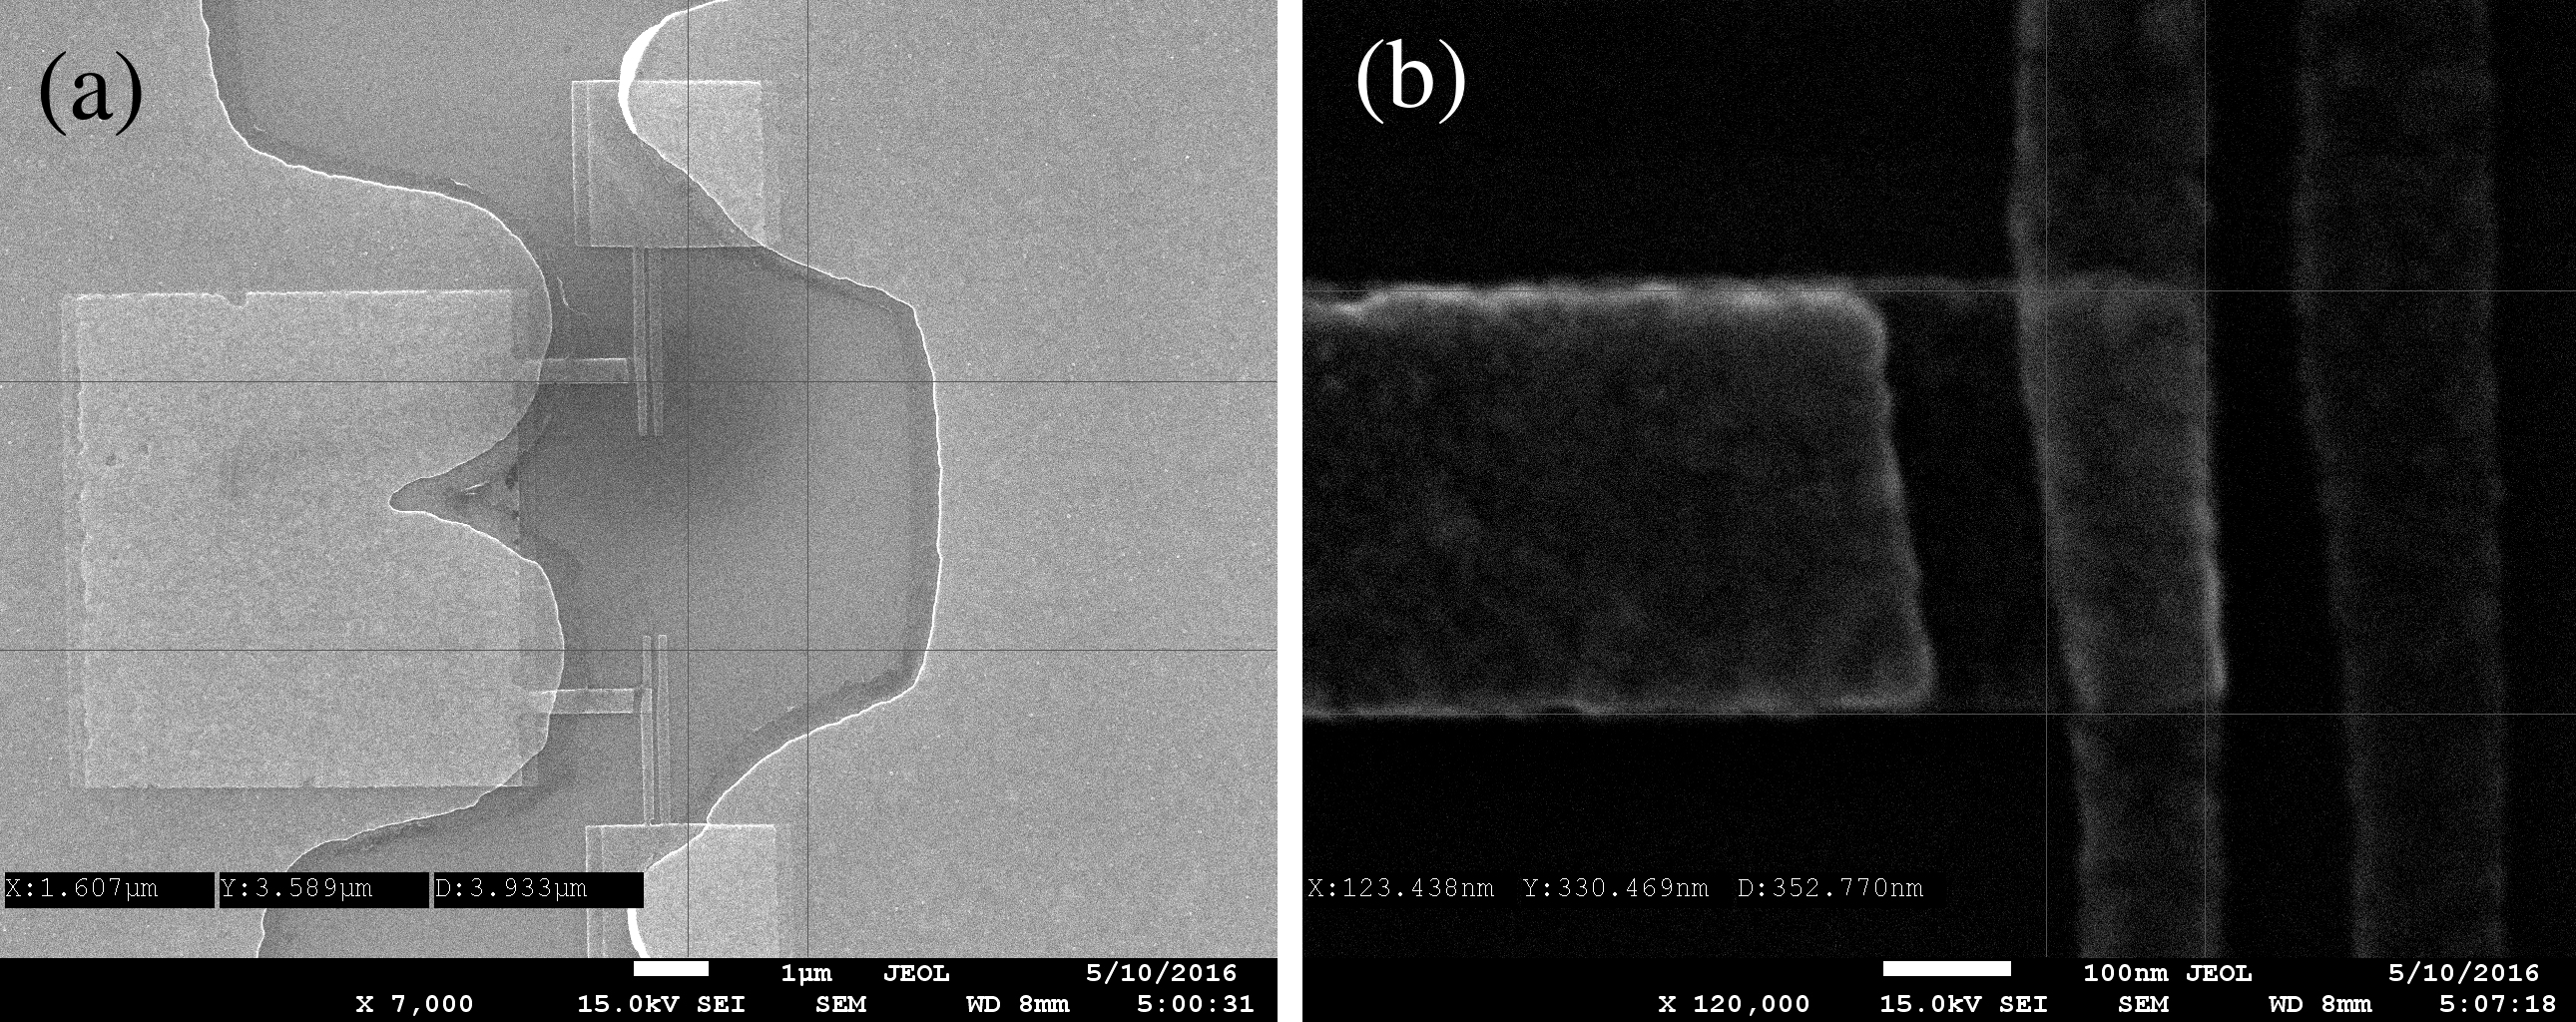
\includegraphics[width=0.9\textwidth]{X_mon_JJ_SQUID}
\caption{\textbf{(a)} SEM micrograph of the SQUID of one of the test structures on the chip. One can see that photo- and electron lithography are aligned, however fine structures \autoref{fig:first_chip_design_full}~(c) were not resolved during the second step. \textbf{(b)} Enlarged view on one of the junctions (upper). Its area is approximately $120\times 330\approx 0.4\, \mu m^2$, in the design it's $0.3\,\mu m^2$.} 
\end{figure}

\subsection{Measurement setup}

The sample was measured at ISSP in laboratory of RQC. Cryogenic equipment was represented by BlueFors LD250 dilution refrigerator, with base temperature of 16 mK. The microwave equipment included R\&S ZNB 10 kHz-20 GHz vector network analyser,  Agilent E8257D 100 kHz - 40 GHz analog signal generator. The sample was flux biased using Keithley 6221 current source.

Microwave line was thermalized with 60 dB of attenuation, additional 20 dB of attenuation were introduced on a directional coupler which added the second tone from the $\mu$-wave source. After leaving the sample the signal passed through two isolators and a hybrid coupler, which was used before to measure two samples during single cooldown. Finally, the signal was amplified with 4-8 GHz LNF amplifier at 4 K and a with a room-temperature amplifier.

The sample holder that was used was designed for 10x10 mm chips, so the bondwires had a relatively large length of 1 mm which of course deteriorated the overall transmission. Chip lay directly on the copper disk of the bottom part of the sample holder with no hole carved under it. Around the sample holder a superconducting coil was wound which has been supplied using the current source mentioned above.

The magnetic shielding of the sample holder was achieved via a cryoperm shield. A superconducting shield was not installed in this run due to the lack of space inside the magnetic shield, which may have influenced the noise background.


\subsection{Characterization of the resonators}

As a first step of characterizing the sample a study of the resonances was performed. In \autoref{fig:first_resonators_general} the power transmission through the cryostat is shown. In can be seen that in overall the transmission level is at approximately $-35$ dB. As long as the amplifiers add 60 dB the directional coupler and the hybrid coupler subtract 23 dB, it can be inferred that the sample in the sampleholder itself has approximately -10 dB transmission. This should be improved with better impedance matching to reduce noise. Secondly, there is a clear 300 MHz-wide dip in the transmission around 6.2 GHz, which should also be eliminated.

\begin{figure}[h]
\centering
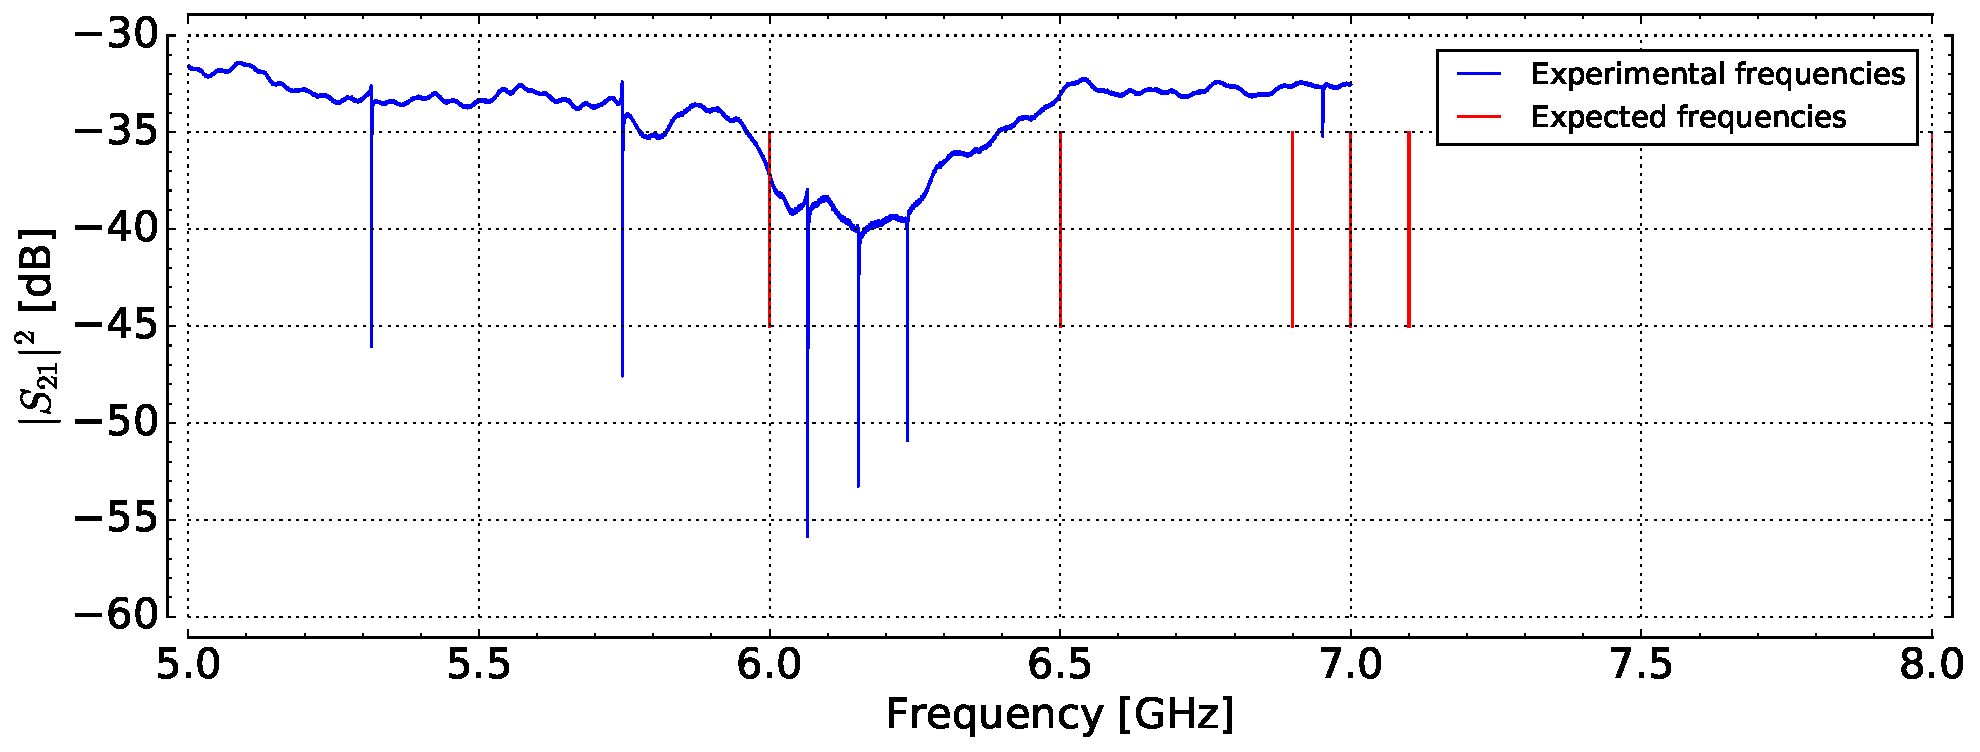
\includegraphics[width=\textwidth]{xmon-first-try_general15x5}
\caption{General view of the resonances. All six resonances are visible, however shifted far down in frequency. This shift is due to a mistake in the design which didn't compensate for the ``claw'' couplers at the resonator ends.}
\label{fig:first_resonators_general}
\end{figure}

All resonators are functional which can be seen from the presence of six sharp dips in transmission. The frequencies at which the dips occur are significantly lower than expected because there was a flaw in the macro code which draws the design. The frequency compensation routine made specifically to calculate the frequency shift\cite{Sank2014} caused by the ``claw'' coupler at the end of the resonator was not executed, so the length of the resonators became larger than it should have been. At higher frequencies the phase shift of the ``claw'' is larger so the frequency discord is larger there.

Below the results obtained using the \textit{circlefit}\cite{probst2015} fitting method are presented. Each peak from \autoref{fig:first_resonators_general} was enlarged and scanned with a fine resolution and averaged to reduce noise (more averages on low and less on high powers). Then for each power complex $S_{21}$ data for each scan area around a resonance was recorded.

After all of the data had been obtained, the fitting procedure has been applied for every scan at each power. The full fitting process is described in depth in the original publication\cite{probst2015}. In practice the whole algorithm is encapsulated in several function calls of the library called \textit{resonator tools} that the authors have kindly provided via \href{https://github.com/sebastianprobst/resonatortools}{GitHub}. Fitting results are summarized in \autoref{fig:first_q_factors}.

\begin{figure}[t]
\centering
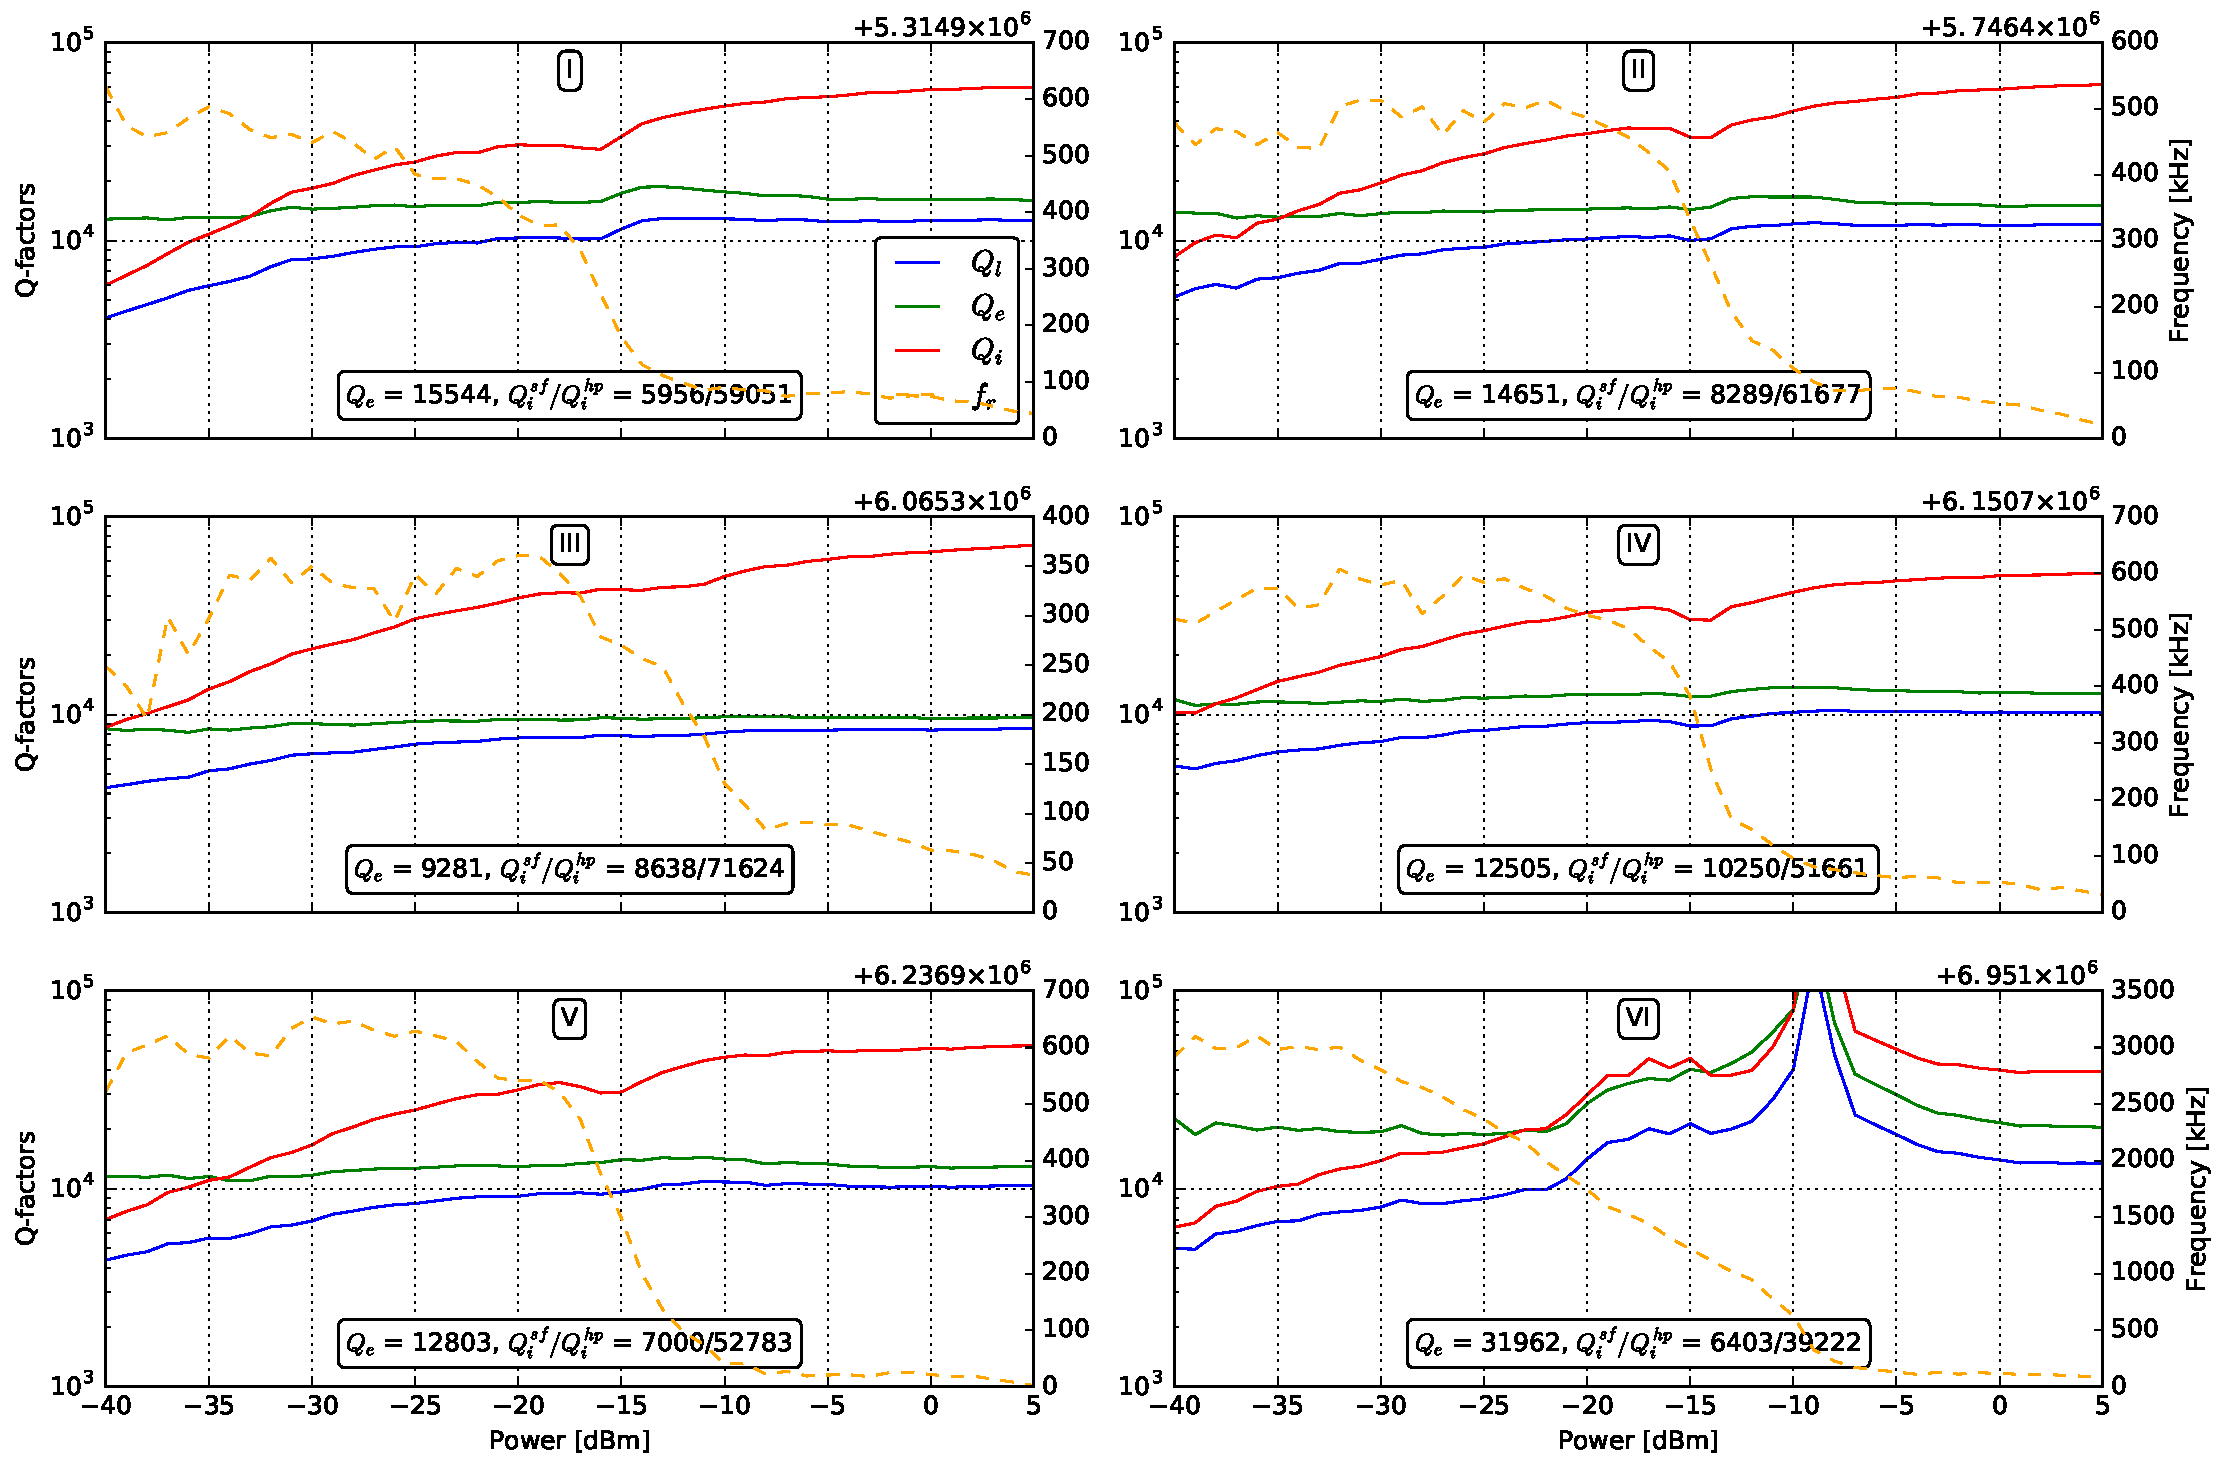
\includegraphics[width=\textwidth]{q-factors-and-freqs_xmon_first_try}
\caption{Various quality factors and frequencies depending on radiation power. Single photon limit is near -40 dBm on the VNA summed with 80 dB of attenuation, saturation limit near 5 dBm on the VNA. All devices show standard behaviour except for the VI\textsuperscript{th} which loses its shape and cannot be fit correctly at powers above -20 dBm.}
\label{fig:first_q_factors}
\end{figure}

It is well-known\cite{wang2009} that for superconducting microwave resonators the internal quality factor experiences an increase in value when probed with higher power. This effect is believed to occur due to the presence of two-level defects or two-level systems (TLS) with a dipole moment in the areas of high electric fields which resonator creates. As long as TLSs have same frequency as the measured resonator and coupled strong enough, they will drain excitations from the resonator. However TLSs can only accommodate only one photon at a time; thus, at high probe powers they saturate and do no more participate in resonator relaxation. Therefore, an increase of the internal Q-factor is observed when the resonator is driven with strong microwave fields.

When the resonator is coupled to a weakly nonlinear quantum system like transmon its quality factor will depend strongly on the coherence time of the qubit when their frequencies are close (thus on the flux bias). Therefore, possibly the low (usual $Q_i$ values for similar Al devices are around 3$\cdot 10^4$) internal quality factor values of the resonators at single-photon level are determined by high dissipation in the qubits that were not detuned far enough in frequency.

\begin{figure}
\centering
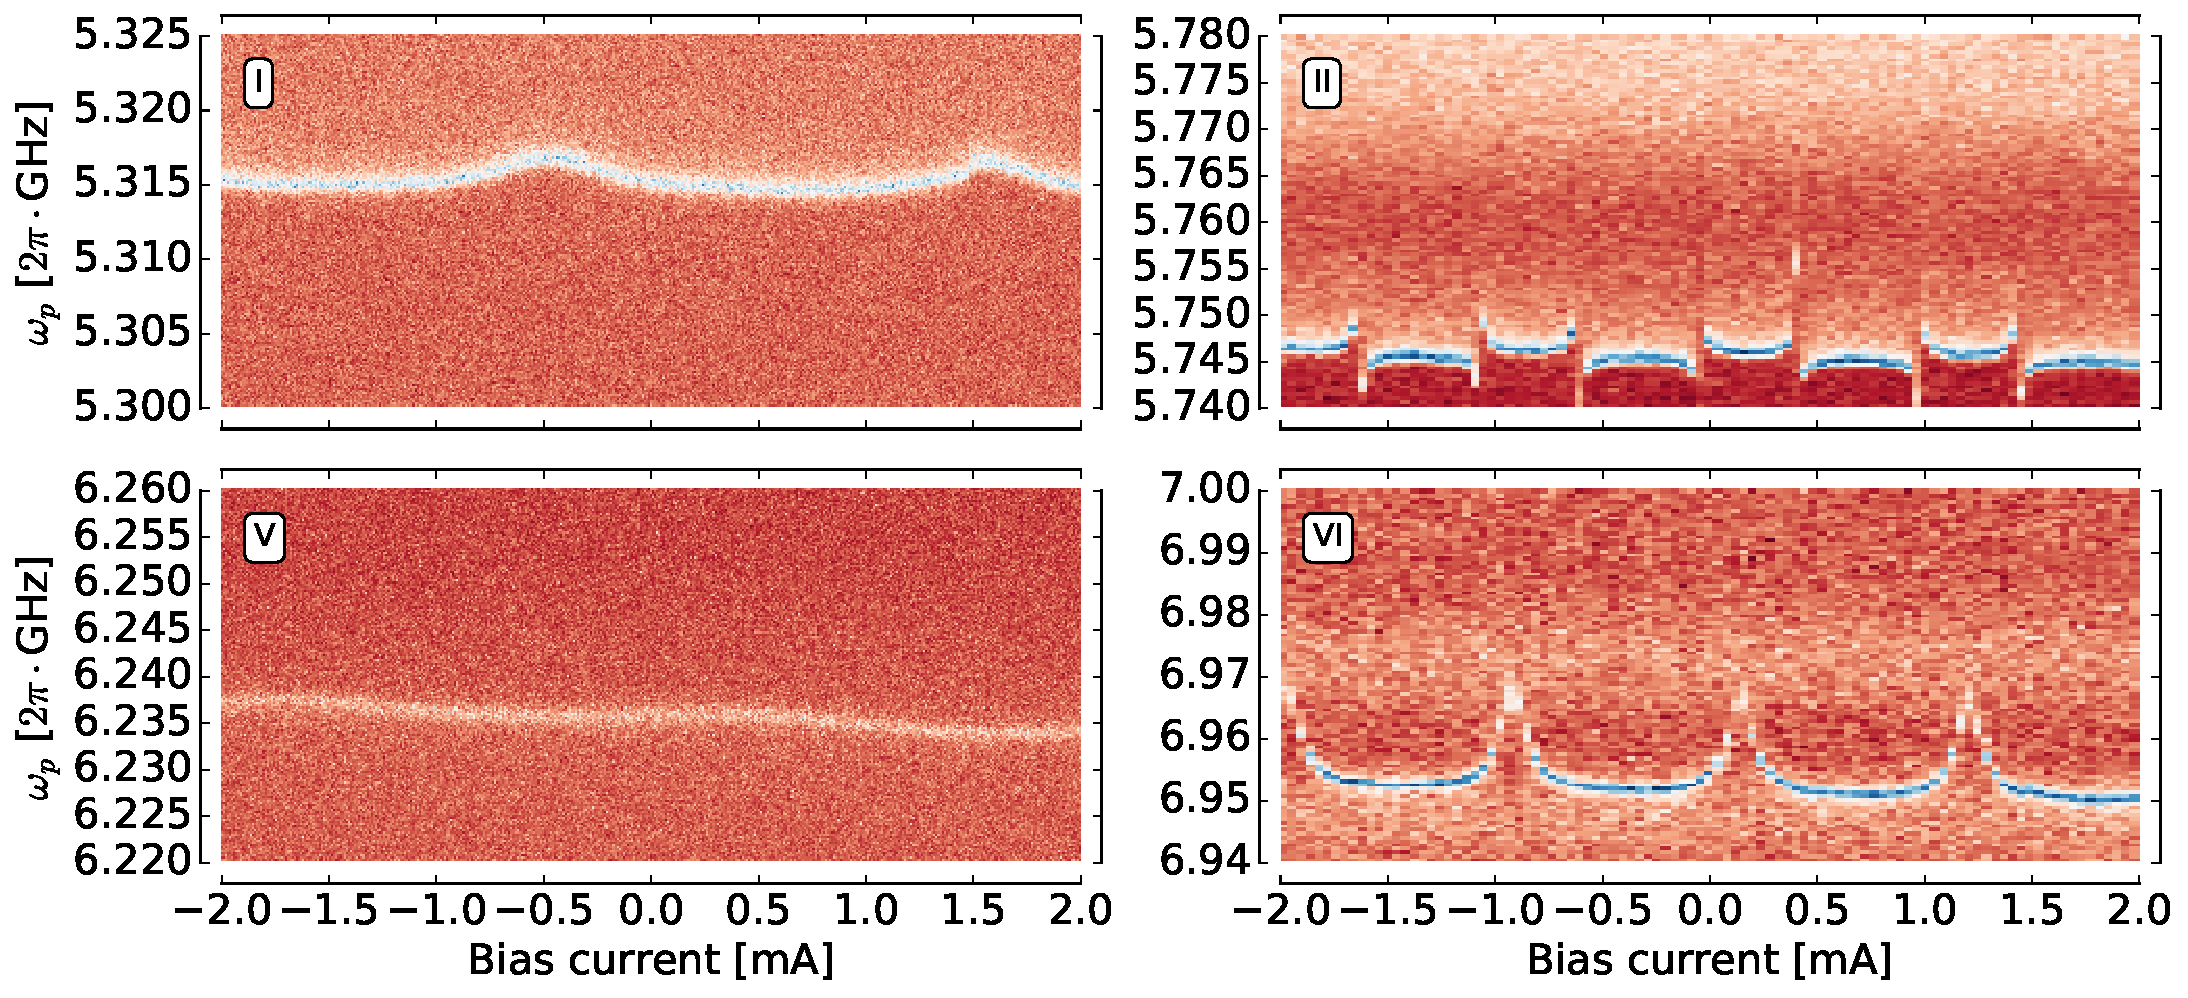
\includegraphics[width=\textwidth]{first_resonators_on_flux}
\caption{Magnetic field influence on frequencies of four devices. Resonators III and IV didn't demonstrate any significant dependence on flux (not shown here).}
\label{fig:first_resonators_on_flux}
\end{figure} 

\subsection{Characterization of the whole cQED systems}

From six systems on the chip only three were studied in detail partly due to lack of time and partly because the overall picture was more or less clear at that point. Firstly the behaviour of the resonators was investigated when the flux bias was being changed. This measurement revealed obvious periodic frequency oscillations in four devices from six, see \autoref{fig:first_resonators_on_flux}. The other two devices didn't show any noticeable periodic flux dependence because one of the qubits (III) had a broken SQUID and the other (IV) probably was much lower in frequency than its resonator.

Firstly system II was measured as long as it has shown the most prominent flux response of all. Then system VI was investigated and, finally, system I. For each of them a two-tone spectroscopy was performed and for II and VI a high-resolution single-tone one as well. Then the data was used to fit the parameters in the model \eqref{eq:hamiltonian} described in \autoref{sec:cQED}. Accordingly, the graphs that are shown below are composed of the experimental spectra overlayed with theoretical curves obtained from numerical solution of the corresponding eigenproblems.

\subsubsection{System II}

\paragraph{Model.} Below all the experimental data will be provided for system II along with theoretical fits of the spectral lines that were observed using the model \eqref{eq:hamiltonian}. Model parameters were fit based on all data on this system and are same for all figures in this section. Before turning to the comparison of the theoretical predictions and experimental results it would be useful to present the model parameters used for fitting which are summarized in \autoref{tab:first_II_params}.

\begin{table}[h]
\centering
\begin{tabular}{l|c}
Parameter & Value \\
\hline 
$C_\kappa$ & 0 fF \\
\hline
$C_g$ & 1.9 fF \\
\hline
$C_q$ & 95 fF \\
\hline
$E_C$ & 200 MHz
\end{tabular}~
\begin{tabular}{l|c}
Parameter & Value\\
\hline
$C_r$ & 444 fF \\
\hline
$L_r$ & 1.72 nH \\
\hline
$I_{C, \Sigma}$ & 69.5 nA \\
\hline
$E_{J, \Sigma}$ & 34.5 GHz
\end{tabular}
\caption{Values of the main parameters defining the spectrum of the model \eqref{eq:hamiltonian}.}
\label{tab:first_II_params}
\end{table}

From these values it's possible to calculate the coupling strength $g \approx 19.6$ MHz between the qubit and the resonator, bare qubit frequency of $\omega^{(0)}_{ge}/2\pi = 7.3$ GHz and bare resonator frequency $\omega^{(0)}_r = 5.758$ GHz. In the coupled system these values are shifted strongly, $\omega_{ge}/2\pi = 7.23$ GHz and $\omega_r = 5.746$ GHz. These shifts are so large (much greater than what would be predicted by the usual dispersive shifts) because of the large value of the Xmon capacitance. Usually cQED systems are treated in the limit of large $C_r \gg C_q, C_g, C_\kappa$ and in this case factors in the terms $\mathcal{\hat H}_q, \mathcal{\hat H}_r $ from \eqref{eq:hamiltonian} can be reduced to their bare uncoupled values. This means the only difference from the uncoupled case is the term $\mathcal{\hat H}_i$, which defines the shifts from the uncoupled frequencies, which are in this case by definition equal to the dispersive shifts. In the studied case $C_q \approx 0.25\, C_r$ and cannot be neglected; thus, the interacting systems are not the same as before coupling, and only the full model \eqref{eq:hamiltonian} taking account of all capacitances can be used to obtain correct results. Despite that after acquiring the new parameters for the interacting systems from \eqref{eq:hamiltonian} the dispersive shifts may be calculated as usual.

The flux normalization on the x-axis was done using data from \autoref{fig:first_resonators_on_flux}~(II) knowing the fact that $\Phi_0$ should be the period of the pattern and that zero flux point is situated at the center of one of the lower branches.

Below in the description of the figures a bit different notation for the transition frequencies may be used than those which denote the theoretical curves on the legends of the graphs. This is due to the fact that in the presence of coupling the qubit spectrum $\omega_{ge}(\Phi_{ext})$ is shared between transitions $\omega_{01}(\Phi_{ext})$ and $\omega_{02}(\Phi_{ext})$ of the full Hamiltonian, so when we say $\omega_{ge}(\Phi_{ext})$ we imply $\omega_{01}(\Phi_{ext})$ and $\omega_{02}(\Phi_{ext})$ for the cases of $\Delta_\omega > 0 $ and $\Delta_\omega < 0$, respectively.

\begin{figure}
\centering
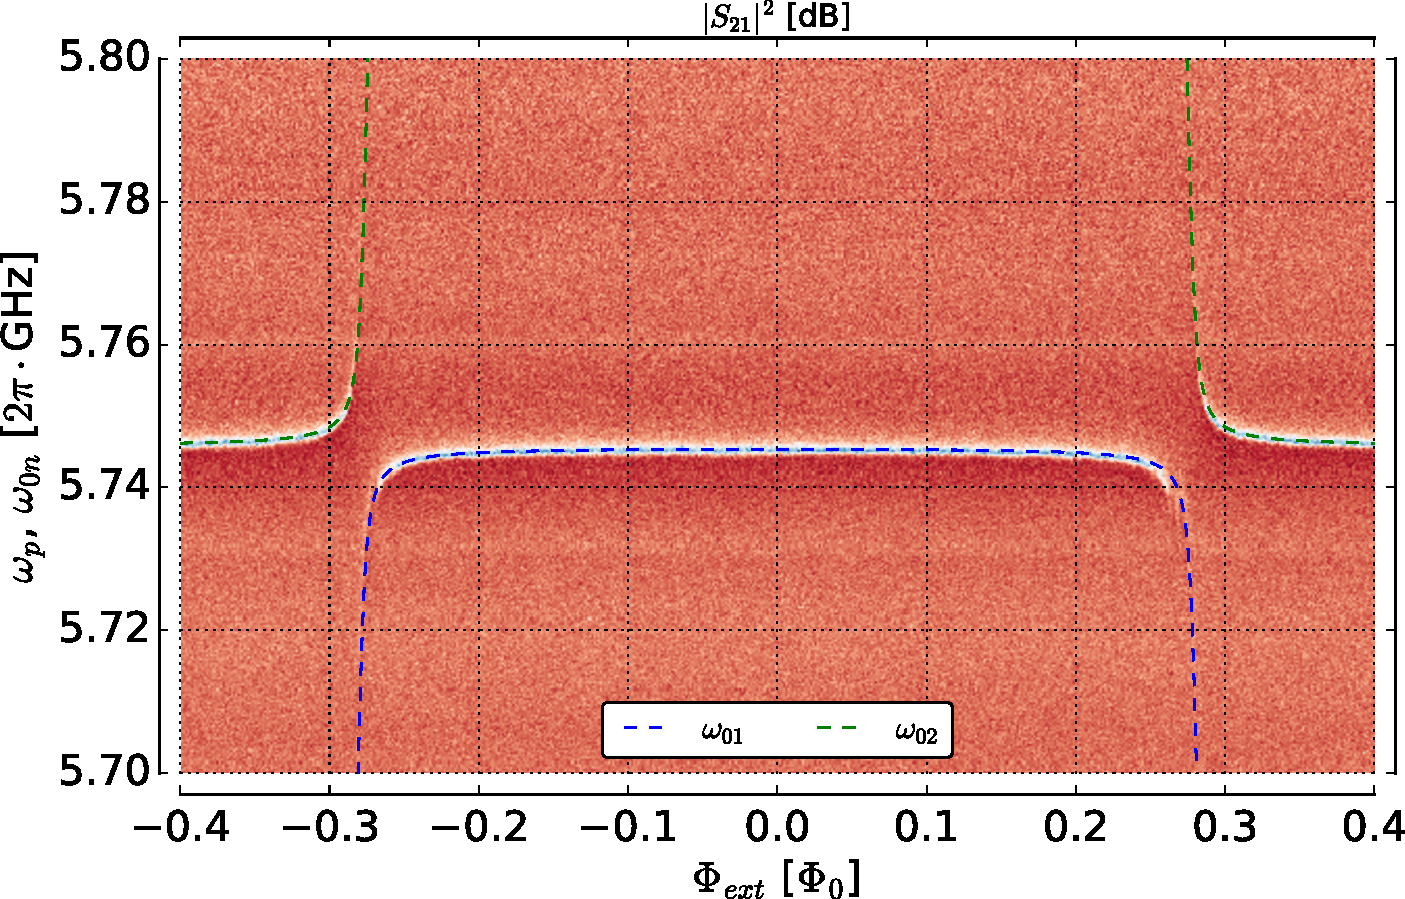
\includegraphics[width=0.9\textwidth]{first_II_anticrossing_fit}
\caption{Anticrossing spectrum of system II with fitting lines obtained by numeric calculation from the model\eqref{eq:hamiltonian} (z-axis normalized). It can be seen that lower branch has some artefacts near the anticrossings which are caused by multiphoton and sideband transitions, signifying that probe power was not at single-photon level. The x-axis is normalized to one flux quantum through the SQUID of the Xmon.}
\label{fig:first_2nd_res_anticrossing}
\end{figure} 

\paragraph{Anticrossing spectrum.} Firstly, a high-resolution scan of one of the anticrossings from \autoref{fig:first_resonators_on_flux}~(II) was obtained. The power level on the VNA was set to -40.0 dBm, which means around -120 dBm at the sample. It is presented in \autoref{fig:first_2nd_res_anticrossing}. It can be seen that a really good agreement between experiment and theory was attained. However there are some discrepancies that can be pointed out: a slight asymmetry of the left and right anticrossings and the reduced brightness of the main branch $\omega_{01}$ on the right. It can be seen clearly from the data that additional multi-photon transitions or sidebands are visible similar to what have been observed before\cite{bishop2009} which indicates that the power was higher than at the single-photon level. Theoretical curves for those transitions were not displayed because the picture becomes too crowded. It is not clear why this effect is stronger in the right anticrossing than in the left one. Further investigation is needed, because at that cooldown due to the setup limitations measurements at lower power were too time consuming because of the low transmission.

\begin{figure}
\centering
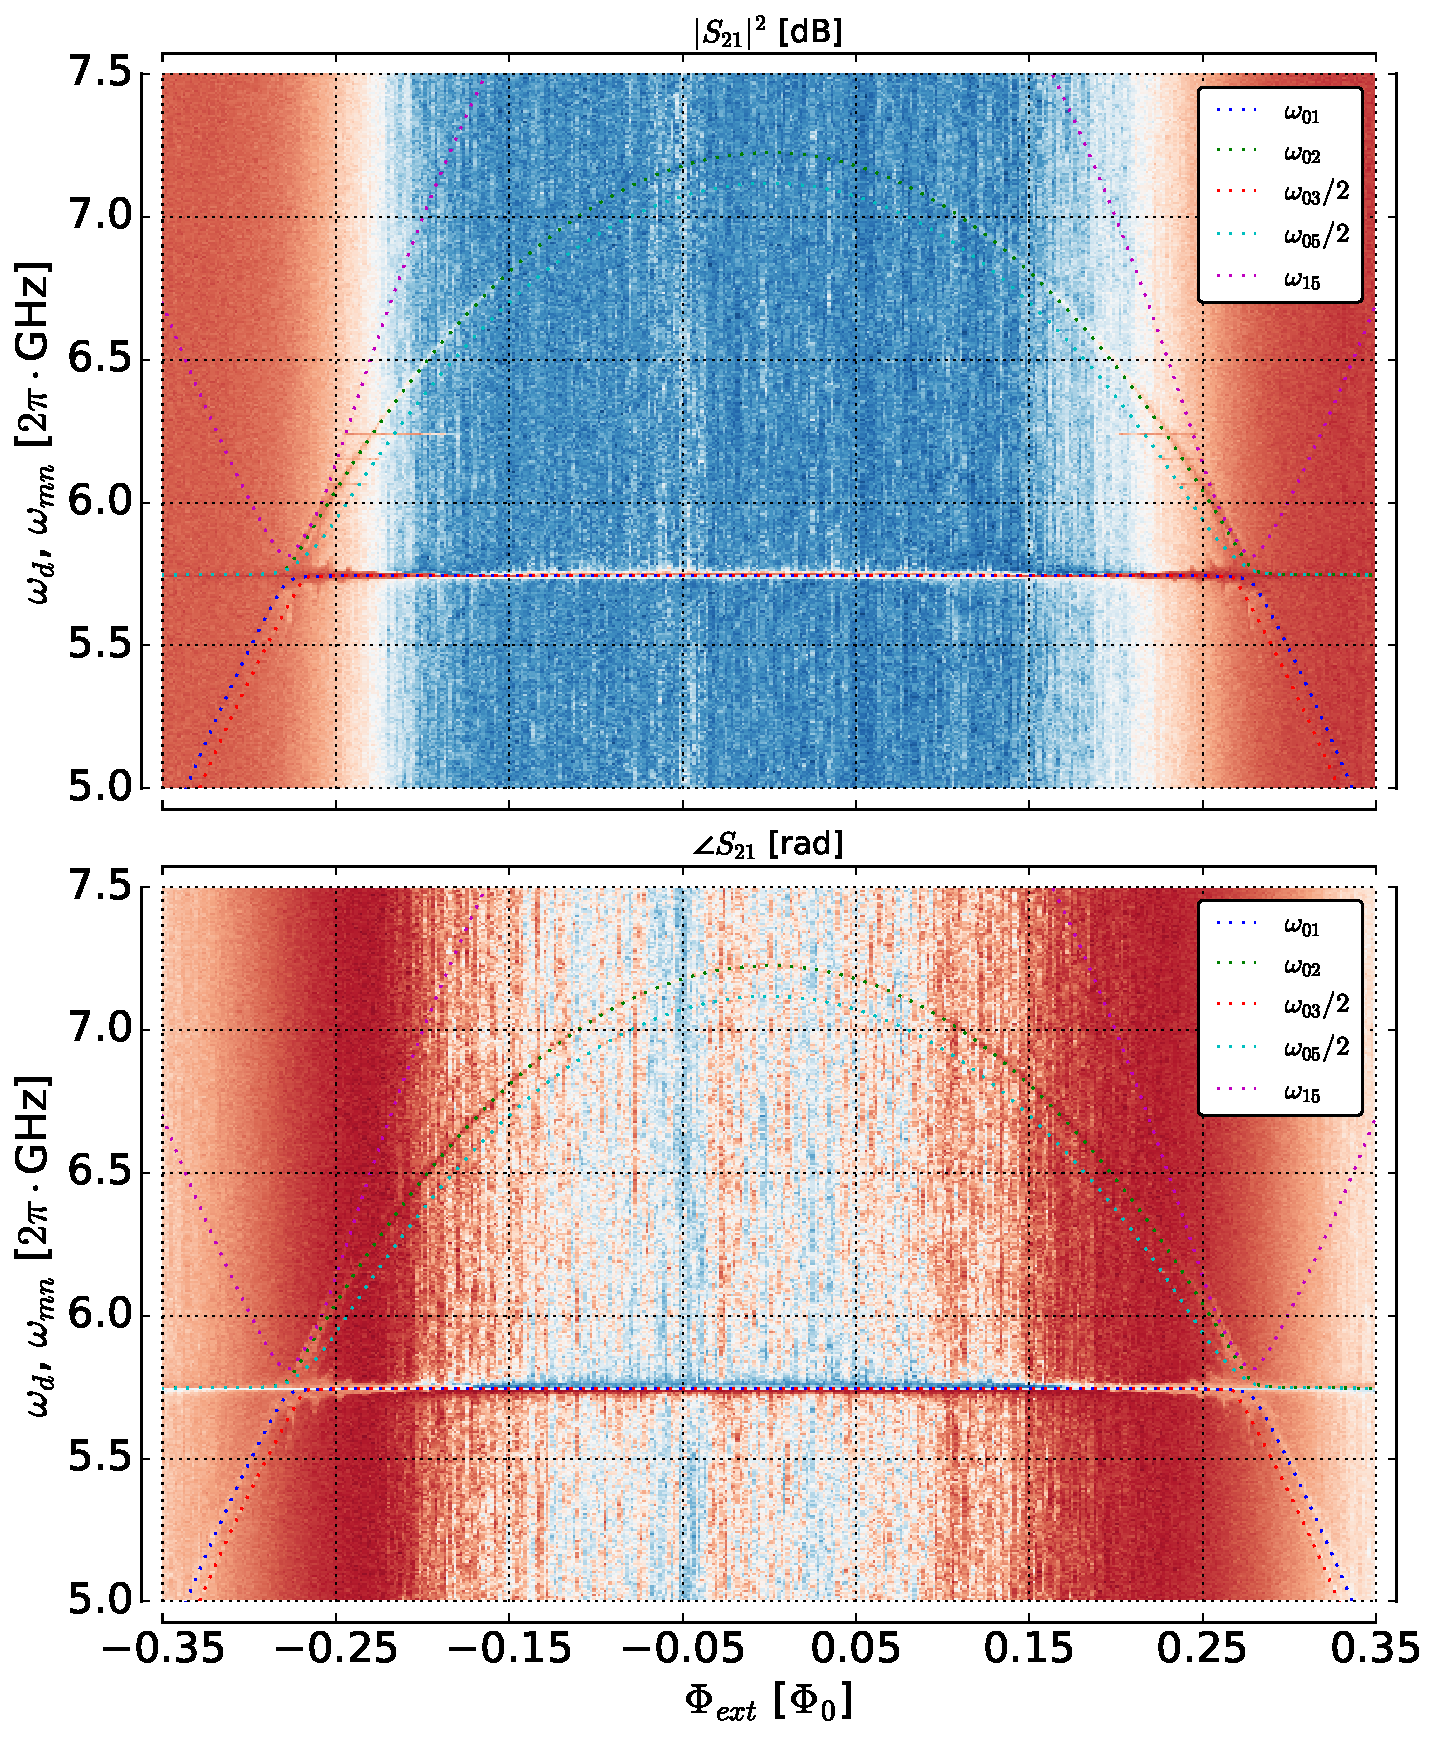
\includegraphics[width=.9\textwidth]{first_II_2tone_fit}
\caption{The two-tone spectrum of system II at -20 dBm power level on the $\mu$-wave source with fitting lines obtained from the model \eqref{eq:hamiltonian}. Various transitions are visible, most pronounced are the horizontal resonator $0n$ transition, the hyperbolic qubit $ge$ transition ($\omega_{01},\ \omega_{02}$) and lower branch of the hyperbolic two-photon $gf$ transition ($\omega_{03}/2$). Also a sideband $\ket{1,g}\rightarrow \ket{0,f}$ is visible ($\omega_{15}$).}
\label{fig:first_II_2tone}
\end{figure}


\paragraph{Two-tone spectroscopy.} Next measurement was a standard two-tone spectroscopy. The results of such measurement at different second tone powers are presented. Firstly, the lowest possible power (-20 dBm) scan was acquired, it is shown in \autoref{fig:first_II_2tone}. It was not possible to set a lower power with the step attenuator of the $\mu$-wave source, however for studied system that power was low enough to observe only single-photon processes without apparent multi-photon transitions and sidebands around the qubit's degeneracy point. However due to the fact that the second tone was introduced from the feedline through the resonator the effective driving power was increasing when the qubit-resonator detuning was decreasing; thus, some secondary transitions become visible near the anticrossing regions. For example, a sideband transition which uses one photon from a resonator and one photon from the incident microwave radiation ($\omega_{15}$) is vaguely visible above the resonator line and a two-photon transition $\omega_{gf}/2$ is clearly visible below it.

\begin{figure}
\centering
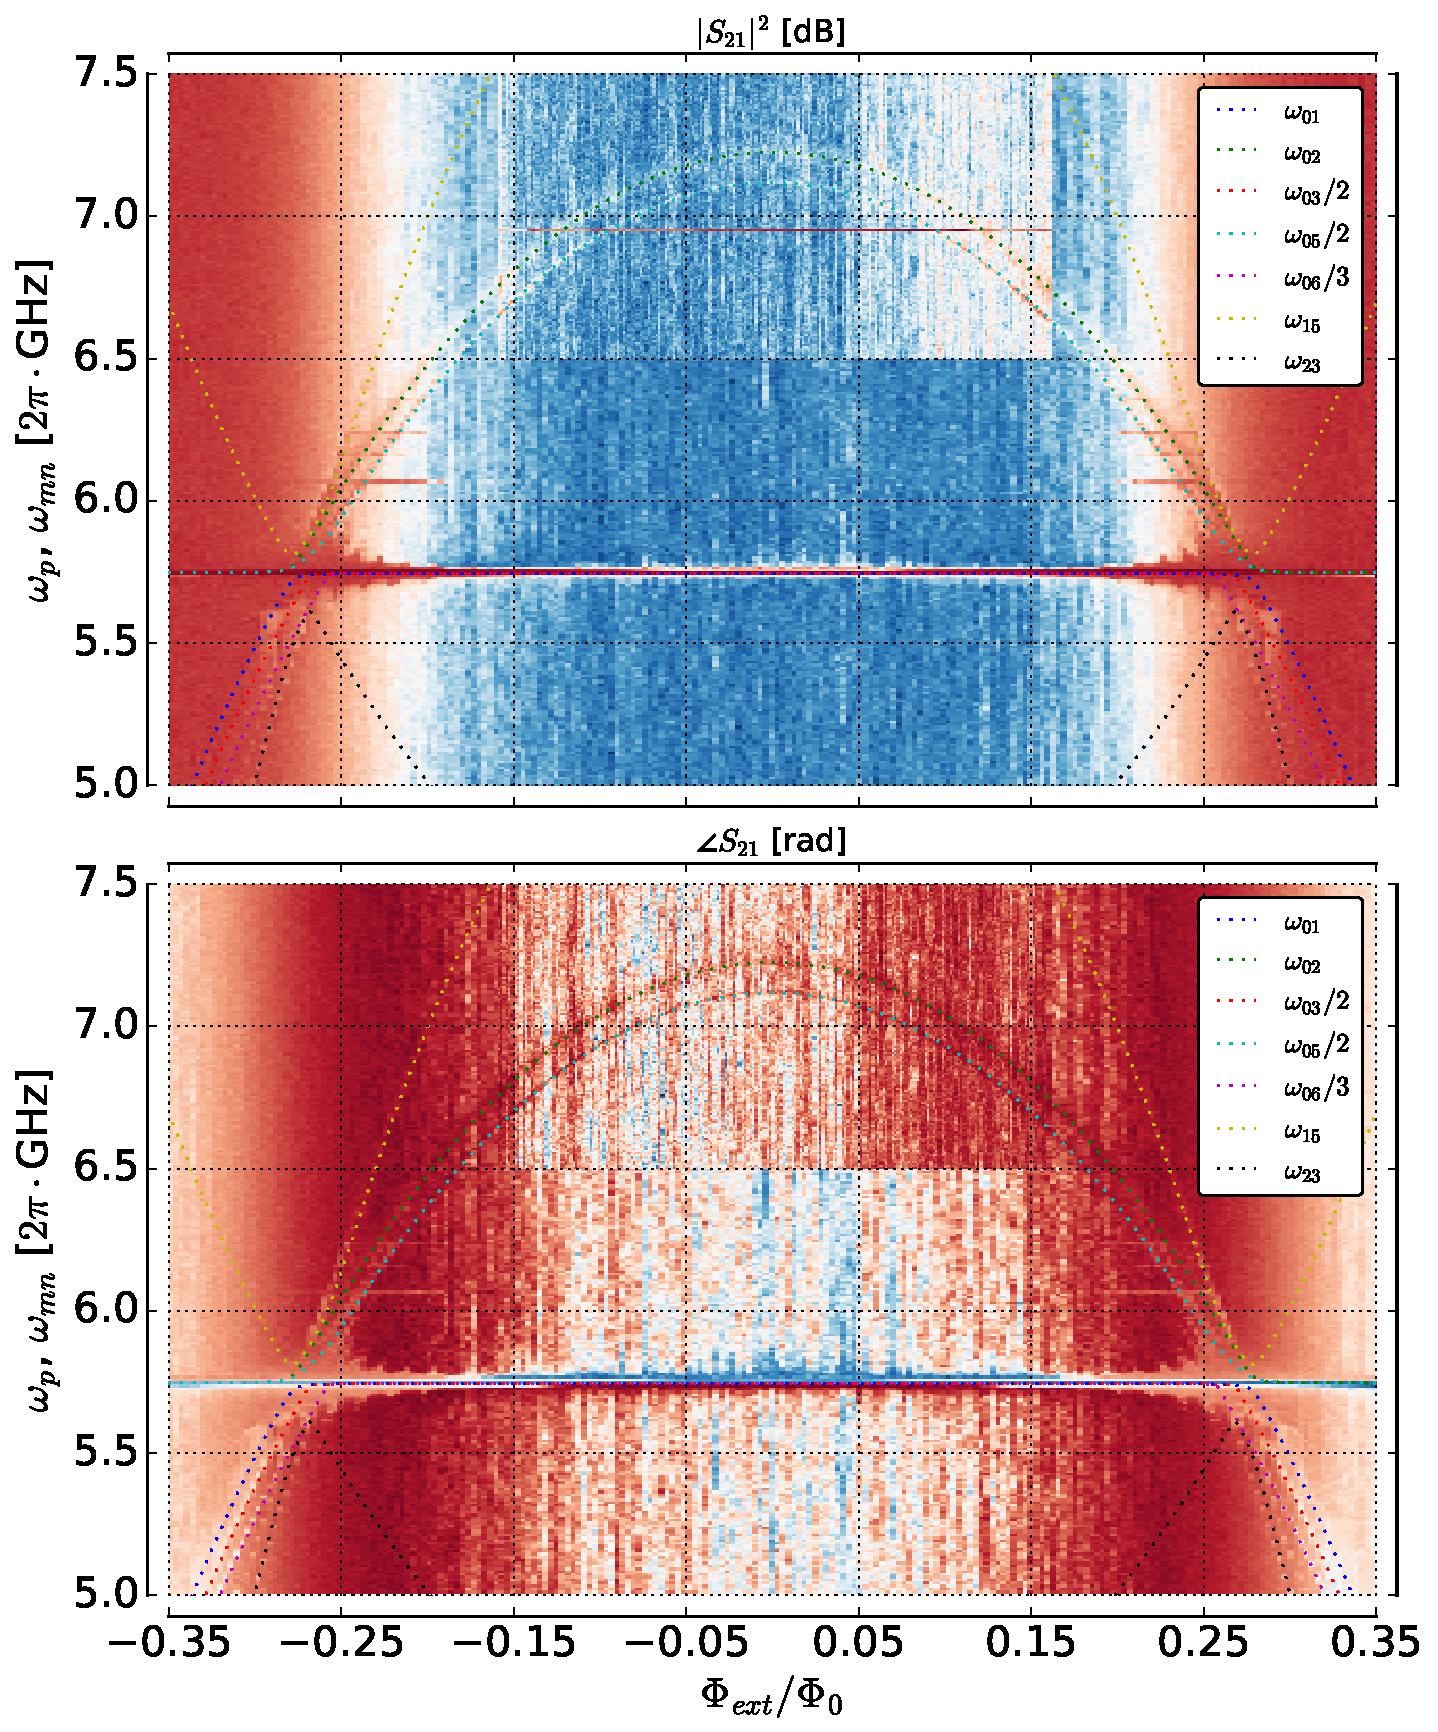
\includegraphics[width=.9\textwidth]{first_II_2tone_higher_power_fit}
\caption{The two-tone spectrum of system II at -10 dBm power level on the $\mu$-wave source with fitting lines obtained from the model \eqref{eq:hamiltonian}. More transitions are visible, new compared to \autoref{fig:first_II_2tone} are the upper branch of the two-photon $gf$ transition ($\omega_{05}/2$), the lower branch of the three-photon $gd$ transition ($\omega_{06}/3$) and also the lower branch of the sideband $\ket{1,g}\rightarrow \ket{0,f}$ ($\omega_{23}$).}
\label{fig:first_II_2tone_hp}
\end{figure}

If the power of the second tone is increased, the probability of the transitions with lesser matrix elements also rises allowing to see these transitions more clearly. Such measurement yields a spectrum as in \autoref{fig:first_II_2tone_hp}. It was done at -10 dBm; thus, a power 10 times higher than in the previous case was sent at the sample. Now the two-photon hyperbolic line $\omega_{gf}$ under the main one $\omega_{ge}$ is clearly visible (the upper complementary branch $\omega_{05}/2$ of the previously visible transition $\omega_{03}/2$). The upper branch of the sideband $\ket{1,g}\rightarrow \ket{0,f}$ is visible also, see \autoref{fig:first_II_2tone_zoom_fit} for the scan around $\Phi_{ext}=0$. Also there are two lines below the resonator at the sides of the graph whose origin is not clear. One of them might be the lower branch of that sideband (fit with $\omega_{23}$ in \autoref{fig:first_II_2tone_hp}), however it can be seen that the theoretical line is not very accurate there. The other line which is visible between $\omega_{23}$ and $\omega_{06}/3$ was not fit because no appropriate transition was found. Surely, one should be able to find it but this task looks hard enough to give it up.

	
\begin{figure}
\centering
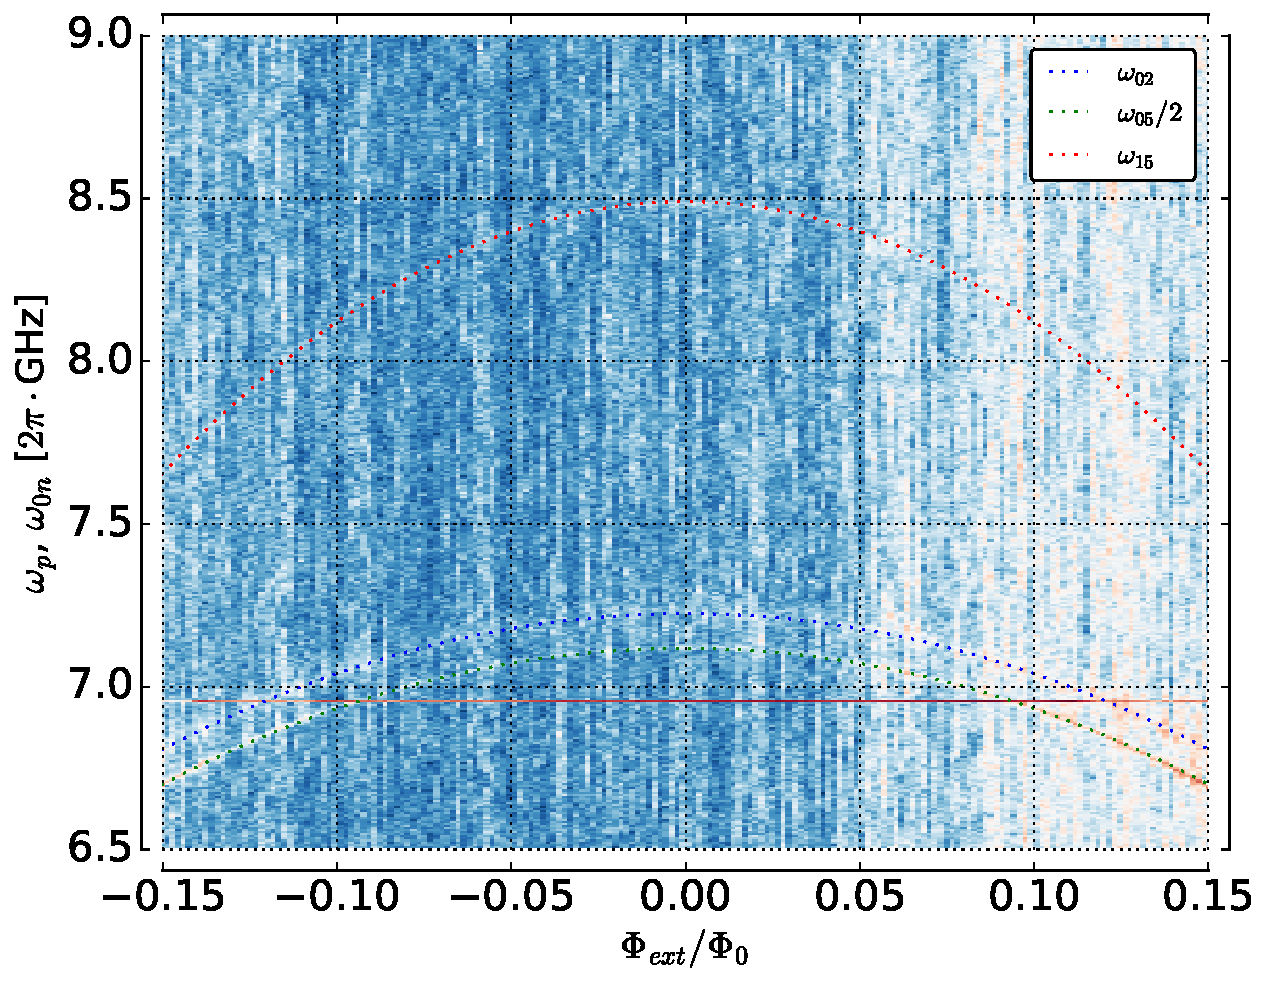
\includegraphics[width=0.8\textwidth]{first_II_2tone_zoom_fit}
\caption{Zoomed area around the main qubit transition $ge$, two-photon transition $gf$ and the sideband transition $\ket{1,g}\rightarrow \ket{0,f}$ with fitting lines. Second tone power was -10 dBm, transmission amplitude is displayed.}
\label{fig:first_II_2tone_zoom_fit}
\end{figure}

Interestingly enough as well as the transition corresponding to the system's resonator some other narrow horizontal transitions are visible. Three of these lines are visible best of all around 6.1 GHz near the qubit line in \autoref{fig:first_II_2tone}~($|S^2_{21}|$) and near 7 GHz in the high-resolution area of \autoref{fig:first_II_2tone_hp}~($|S^2_{21}|$). They correspond to the other resonators which lie higher in frequency. This effect was already observed before but was not thoroughly studied. At this moment it seems that the effect of changed transmission on the probe frequency when the other resonator is resonantly excited with large power (second tone power is 10$^4$-10$^5$ times higher than the probe power) is not due to the coupling of the resonators but due to nonlinear effects or suppressed superconductivity in the Al film itself.

\newpage

\subsubsection{System VI}

\paragraph{Model.} Below all the experimental data will be provided for system VI along with theoretical fits of the spectral lines that were observed using the model \eqref{eq:hamiltonian}. Model parameters were fit based on all data on this system and are same for all figures in this section. Before turning to the comparison of the theoretical predictions and experimental results it would be useful to present the model parameters used for fitting which are summarized in \autoref{tab:first_VI_params}.

\begin{table}[h]
\centering
\begin{tabular}{l|c}
Parameter & Value \\
\hline 
$C_\kappa$ & 0 fF \\
\hline
$C_g$ & 1.8 fF \\
\hline
$C_q$ & 95 fF \\
\hline
$E_C$ & 200 MHz
\end{tabular}~
\begin{tabular}{l|c}
Parameter & Value\\
\hline
$C_r$ & 367 fF \\
\hline
$L_r$ & 1.41 nH \\
\hline
$I_{C, \Sigma}$ & 63.4 nA \\
\hline
$E_{J, \Sigma}$ & 31.5 GHz
\end{tabular}
\caption{Values of the main parameters defining the spectrum of the model \eqref{eq:hamiltonian}.}
\label{tab:first_VI_params}
\end{table}

\paragraph{Anticrossing.} The anticrossing spectrum of the sixth system is presented in \autoref{fig:first_VI_anticrossing_fit}. It can be directly seen that the qubit is very close in frequency to its resonator; thus, the resonator line is bent slightly and the qubit line is looking ordinary. Using the theoretical model \eqref{eq:hamiltonian} these two lines were fit, and there's a good agreement between theory and data. It can be seen that at the degeneracy point, where the qubit is closest in frequency to the resonator, the resonator line becomes dimmer; it indicates that the qubit is less coherent than the resonator, reducing its Q-factor when approaching resonant interaction.

\begin{figure}
\centering
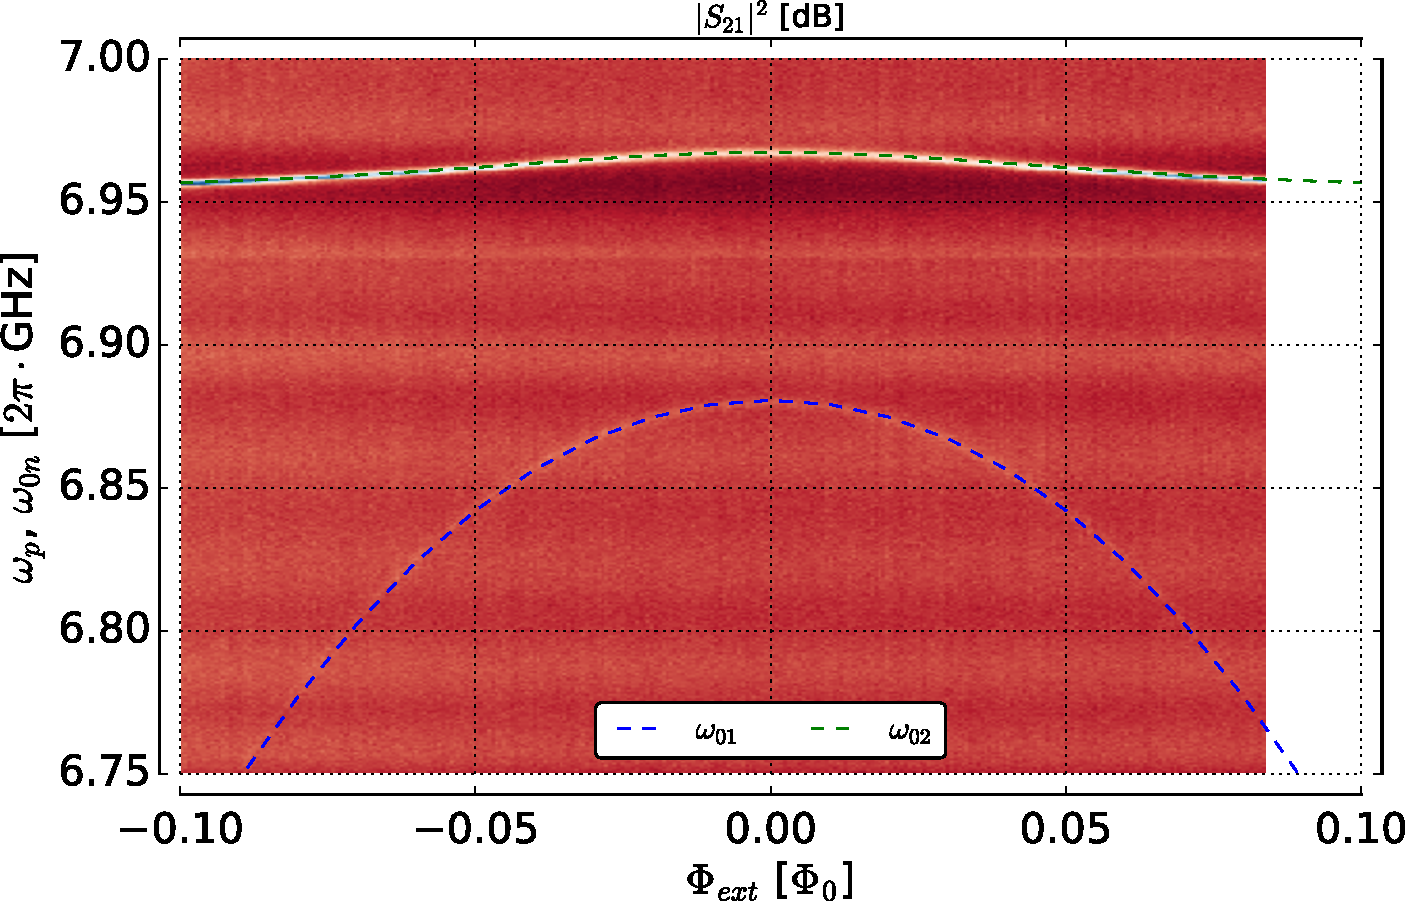
\includegraphics[width=0.9\textwidth]{first_VI_anticrossing_fit}
\caption{Anticrossing spectrum for the 6$^\text{th}$ system (z-axis normalized) with fitting lines obtained from the model \eqref{eq:hamiltonian}. }
\label{fig:first_VI_anticrossing_fit}
\end{figure}

\paragraph{Two-tone spectroscopy.} The results of the two-tone spectroscopy are presented in \autoref{fig:first_VI_2tone_fit}. It was performed at the lowest possible power of -20 dBm on the $\mu$-wave source, yet, due to a very small detuning of the qubit at the degeneracy point, the power in

\begin{figure}
\centering
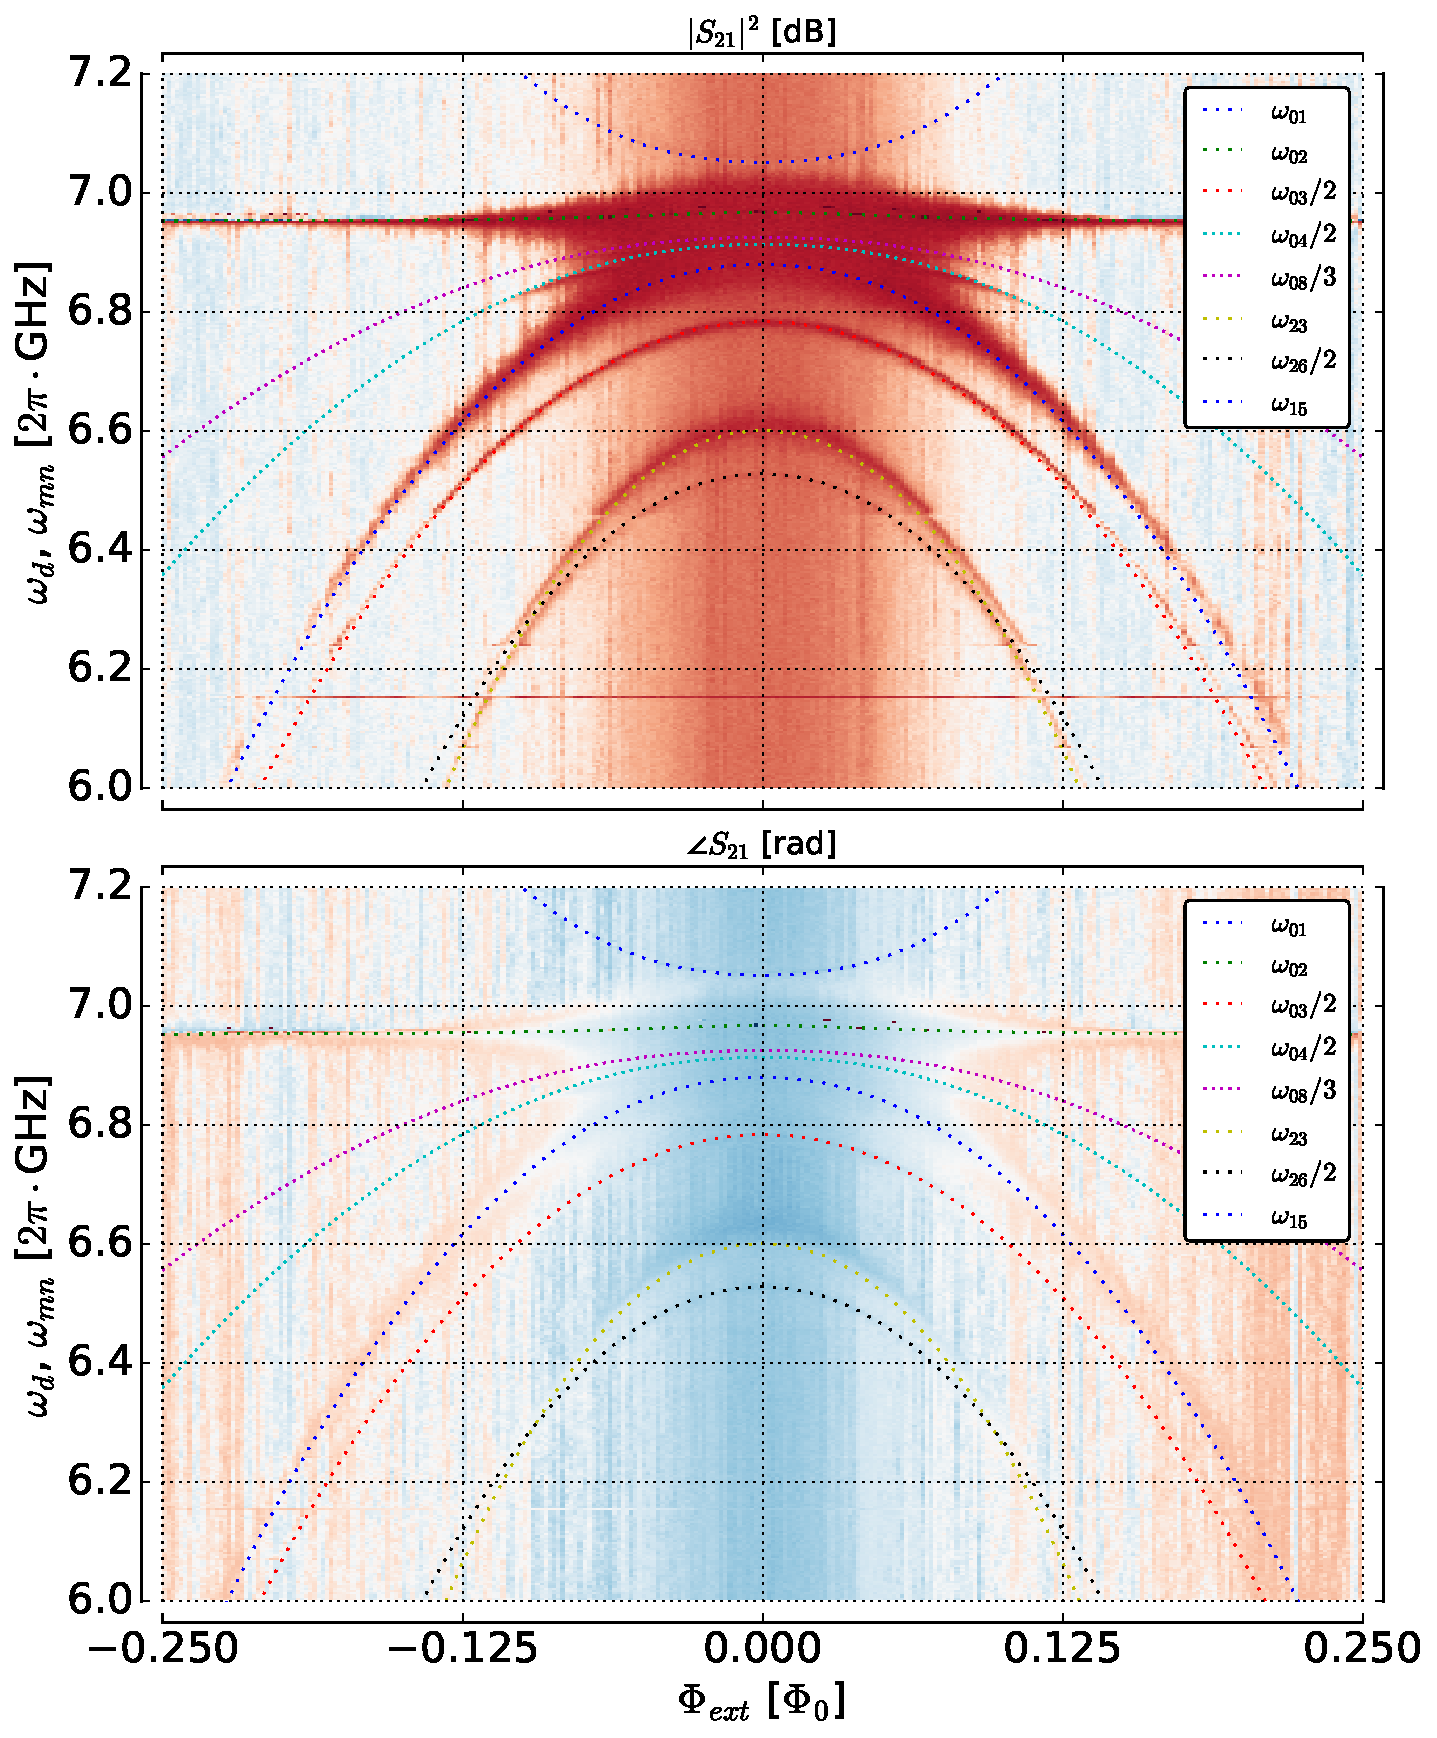
\includegraphics[width=.9\textwidth]{first_VI_2tone_fit}
\caption{Two-tone spectrum of the 6$^\text{th}$ system (z-axis normalized) at -20 dBm on the $\mu$-wave source with fitting lines obtained from the model \eqref{eq:hamiltonian}. As long as the qubit is very close to the resonator in frequency the effective driving power on it is very high, and thus a lot of sideband and multiphoton transitions are visible.}
\label{fig:first_VI_2tone_fit}
\end{figure}

\newpage

\section{On-chip control lines testing design}

\subsection{Geometry and parameters}

The second design that was developed was intended to test the properties of the control lines, i.e. flux bias lines and microwave driving lines, implemented on the chip. The design is presented in \autoref{fig:second_design_full} where some of its key features are highlighted. It's 10x5 mm.

\begin{figure}[h!]
\centering
\includegraphics[width=0.7\textwidth]{chip_design2}
\includegraphics[width=0.7\textwidth]{chip_design2_zoom}
\caption{\textbf{(a)} Large-scale image of the lines testing design. The chip (8x4 mm) consists of eight $\lambda/4$ CPW resonators coupled capacitively to the feedline, six low-Q$_e$ with Xmon qubits at the open end and two high-Q$_e$ with no qubits. \textbf{(b)} Zoomed area around one of the qubits, showing the microwave antenna configuration. \textbf{(c)} Zoomed area around another qubit, showing the flux bias line. \textbf{(d)} Zoom around one of the qubits' SQUIDs. Pink areas denote the part of the mask which produces the SQUID and should be patterned with higher resolution.}
\label{fig:second_design_full}
\end{figure}

Firstly, differently from the previous design, this design has more resonators, additional two (TI, TII, see \autoref{fig:second_design_full}(a)) were inserted at the ends of the main resonator-qubit array (I-VI). These resonators have high Q$_e$ from their geometry to yield accurate results for possible high internal Q-factors.

Secondly, the frequencies of the devices were changed. The qubits still are all calculated to have the same frequency, but it's now 6 GHz, with $C_\Sigma \approx 80$ fF and $I_{C, \Sigma} = 40$ nA. The size of each junction in the qubit's SQUID is 100x200 nm$^2$. The resonators had frequencies of 7, 7.1, 7.2, 7.3, 7.4, 7.5 GHz for the cQED systems I-VI, and the bare resonators TI and TII had 8 and 8.25 GHz, respectively.

Finally, as the main change made to the design, some coplanar control lines were introduced. For the upper qubits they are microwave antennas, i.e. open-ended coplanar line pieces, to induce transitions while for the lower qubits they are flux-bias lines to change the energy level structure of the devices. The lines were separated in such a way to make the design more fault-tolerant.

Four test structures at the sides of the chip were also included to allow direct DC measurement of the SQUIDs created during the shadow evaporation.


\begin{figure}
\centering
\includegraphics[width=0.6\textwidth]{xmon_al_bmstu_1_in_pcb}
\caption{Bonded Xmon Al BMSTU 1 in the PCB of the sample holder, as seen through the microscope of the bonding machine.}
\label{fig:first_tight_fit}
\end{figure}

\subsection{Implementation and purposes}

The chip Xmon Al BMSTU 1 was made in a single-step process. It had a mask patterned with e-beam in the cleanroom facility at Bauman Moscow State Technical University (add recipe?), and then Al film was shadow-evaporated on Plassys in the RQC lab in ISSP, 25 and 45 nm thick. The substrate used was made of high-resistivity Si ($> 6$ kOhm/cm).

One significant difference about this sample is that in fact it was fabricated with its twin in the center of a larger substrate (15x15 mm) which was previously patterned on the back side with a circular saw to allow the substrate to be cracked around the chips precisely. However, the process wasn't yet mastered, and the twin chip was lost during the separation. But nevertheless, the remaining sample fitted in the PCB cutout really well (see \autoref{fig:first_tight_fit}), and the method will be further improved.


Purposes for the design:
\begin{enumerate}[label=(\alph*), leftmargin=1.5cm]
\itemsep0pt
\item to test resonator Q without qubits

\item to test lines

\item to test again the qubits' basic parameters

\item to test improvement of the noise

\item to test the half-sawing of the sample with following cracking
\end{enumerate}

\subsection{Measurement setup  STUBBED from first chip, needs review}

The sample was measured at ISSP in laboratory of RQC. Cryogenic equipment was represented by BlueFors LD250 dilution refrigerator, with base temperature of 16 mK. The microwave equipment included R\&S ZNB 10 kHz-20 GHz vector network analyser,  Agilent E8257D 100 kHz - 40 GHz analog signal generator. The sample was flux biased using Keithley 6221 current source.

Microwave line was thermalized with 60 dB of attenuation, additional 20 dB of attenuation were introduced on a directional coupler which added the second tone from the $\mu$-wave source. After leaving the sample the signal passed through two isolators and a hybrid coupler, which was used before to measure two samples during single cooldown. Finally, the signal was amplified with 4-8 GHz LNF amplifier at 4 K and a with a room-temperature amplifier.

The sample holder that was used was designed for 10x10 mm chips, so the bondwires had a relatively large length of 1 mm which of course deteriorated the overall transmission. Chip lay directly on the copper disk of the bottom part of the sample holder with no hole carved under it. Around the sample holder a superconducting coil was wound which has been supplied using the current source mentioned above.

The magnetic shielding of the sample holder was achieved via a cryoperm shield. A superconducting shield was not installed in this run due to the lack of space inside the magnetic shield, which may have influenced the noise background.

\begin{figure}[h!]
\centering
\includegraphics[width=0.9\textwidth]{xmon_al_bmstu_1_general}

\includegraphics[width=0.9\textwidth]{xmon_al_bmstu_1(2)_general}

\includegraphics[width=0.9\textwidth]{xmon_al_bmstu_1(3)_general}


\caption{\textbf{(Top)} General view of the resonances. All six resonances are visible, however shifted down in frequency. This shift more or less consistent throughout the devices, and thus it's most probably caused by effective $\epsilon_{Si}$ different from the one used in the calculation. \textbf{(Middle)} General view of the resonances (2$^\text{nd}$ cooldown). Transmission now lower as a 5 dB attenuator was replaced by a 10 dB one. Seven resonances are visible, as the second resonator presumably coupled to something. The shapes of the other peaks also changed. \textbf{(Bottom)} General view of the resonances (3$^\text{d}$ cooldown).  Transmission is 20 dB higher as the directional coupler was altered. Again, six resonances are visible, though some spurious dip is present between devices III and IV, and the shapes changed again.}
\label{fig:second_resonators_general}
\end{figure}


\begin{figure}[h!]
\centering

\includegraphics[width=\textwidth]{q-factors-and-freqs_xmon_al_bmstu_1}

\caption{Various quality factors and frequencies depending on radiation power. Some resonators show interesting dip in internal Q near -25 dBm and significant change in frequency, implying they are coupled to functioning qubits saturation of which causes the effect. Other resonators do not show such features.}
\label{fig:second_q_factors}
\end{figure}

\begin{figure}[h!]
\centering
\includegraphics[width=\textwidth]{q-factors-and-freqs_xmon_al_bmstu_1(2)}
\caption{Same figure for the 2$^\text{nd}$ cooldown. Significant deviations are present in comparison with the first cooldown, both to the greater and to the lower Q-factors on different devices.}
\label{fig:second_q_factors(2)}
\end{figure}

\begin{figure}[h!]
\centering
\includegraphics[width=\textwidth]{q-factors-and-freqs_xmon_al_bmstu_1(3)}
\caption{Same figure for the 3$^\text{d}$ cooldown. The Q-factors degraded completely both for the cQED resonators and the test resonators.}
\label{fig:second_q_factors(3)}
\end{figure}

\subsection{Characterization of the resonators}

The resonators on the sample were measured several times (after each new cooldown) as they seemed to degrade. Indeed, looking at the Q-factors over the cooldowns reveals that the resonators got worse and worse, even if nothing at all was done with the chip.

Before the second cooldown the chip was moved out of the PCB to solder additional SMP connectors on it, and then moved back in. No mechanical damage or contamination was inflicted to it. However, we can see dramatic changes in quality factors of the resonators, some got better and some got worse for unknown reasons (see \autoref{fig:second_q_factors(2)}). Devices II and III got so bad it was impossible to fit them as their widths compare to the S$_{12}$ general roughness features (see \autoref{fig:second_resonators_general} (Top) vs (Middle)).

After that before the third cooldown nothing at all was done to the chip. After the cooldown and before the Q-factor measurement there was an accidental excessive current through the surrounding coil. Though, it didn't change the general appearance of the resonances which was again found different at this cooldown (see \autoref{fig:second_resonators_general} (Bottom)). At this run the Q-factors became unacceptably low (see \autoref{fig:second_q_factors(3)}) at all powers. 


\subsection{Characterization of the cQED systems}

The two systems were possible to study in this sample, I and VI. Others either did not indicate presence of the functional qubits or experience strong flux hopping while tuned via the superconducting coil and don't have the flux bias lines attached to work around this problem. Fortunately, system I has the qubit with the flux bias line and system VI has the microwave antenna, so both these on-chip devices were successfully tested.



\subsubsection{System I}

The system one was biased by the superconducting loop right on the chip. This allows to make wide scans without affecting negatively the resonator with the width limited only by the current source. The periodic spectrum of the anticrossings for system I is displayed in \autoref{fig:second_I_anti}. The pattern is shifted noticeably to the left due to some residual field around the sample.

\begin{figure}[h]
\centering
\includegraphics[width=\textwidth]{second-I-anti}
\caption{Periodic anticrossing picture for the system I (at high power). The current on the current source spans 80 mA and is actually comparable at the endpoints to it's maximum possible output of 105 mA.}
\label{fig:second_I_anti}
\end{figure}

\begin{figure}[h]
\centering
\includegraphics[width=\textwidth]{second-I-spec-lines}

\includegraphics[width=\textwidth]{ge-linewidth}
\caption{Qubit spectrum at 0 dBm on the output of the 2$^{\text{nd}}$ tone generator (left), dependence of the linewidth on the driving power (right) and high-resolution scan of the two-tone peak at -20 dBm (bottom).}
\label{fig:second_I_spec_lines}
\end{figure}


The experiment to determine qubit spectrum and the linewidth at the degeneracy point was also done on the system. The resulting graphs are presented in \autoref{fig:second_I_spec_lines}. On the right plot the spectrum of the qubit is visible; it consists of three lines corresponding to the transitions $ge,\ gf/2$ and $gd/3$ and visible due to the high power of the drive. On the left plot the spectral line width is recorded over the incident power of the drive. It's possible to estimate the linewidth of the bare qubit from the phase 2-tone data (see Section \ref{sec:2tone}). The line experiences significant broadening with increased power; though, at the minimal possible power of -20 dBm it's width is very small, around 0.5 MHz, which allows to set a lower bound of 300 ns on the qubit $T_1$ (assuming that there's no pure dephasing due to the flux fluctuations at the sweet spot and to the excessive population of the resonator as $\delta\omega = \frac{1}{T_1}+\frac{2}{T_2}$).

\subsubsection{System VI}

System VI had an on-chip microwave antenna nearby, but had no flux bias line (see \autoref{fig:second_design_full}), and thus had to be biased by the external coil. With the studied sample this method of biasing was very inconvenient, as even small magnetic field from the coil influenced the resonators tremendously, inducing continuous and discontinuous frequency shifts in them, presumably due to flux creep and hopping. Fortunately, is was still possible to tune the qubit of the VI$^{\text{th}}$ system enough to observe it's spectrum and to test the microwave antenna.

\begin{figure}
\centering
\includegraphics[width=0.7\textwidth]{second_VI_anti}
\caption{Anticrossing of the VI$^{\text{th}}$ cQED system. It can be seen that the picture is not symmetric and   the lines are bent downwards at the ends, as the resonator frequency change was caused not only by the qubit, but also directly by the magnetic field.}
\label{fig:second_VI_anti}
\end{figure}

The anticrossing measured for this system is shown in \autoref{fig:second_VI_anti}. It was hard to measure, though, as the flux hopping was interfering with the tuning of the qubit. The resonator frequency change due to the magnetic field has bent the picture, so it would be impossible to fit it within the model described before. Nevertheless, the spectrum of this qubit was gathered with 2-tone spectroscopy using the microwave antenna and with a second tone driving the resonator. The results are presented in \autoref{fig:second_VI_spec_antenna} for the measurement via an antenna and with an additional tone in the feedline driving the resonators at the qubit's frequency.

\begin{figure}[h]
\includegraphics[width=\textwidth]{second_VI_spec_antenna}
\caption{Two-tone spectroscopy of the VI$^{\text{th}}$ system using the microwave antenna mounted on the chip.}
\label{fig:second_VI_spec_antenna}
\end{figure}

\begin{figure}[h]
\includegraphics[width=\textwidth]{second_VI_spec}
\caption{Two-tone spectroscopy of the VI$^{\text{th}}$ system using the directional coupler to add the second tone to the probe line. The background was subtracted. It can be seen also where the flux jumped abruptly: it happened near 0.5 mA and resulted in a decrease of the field penetrating the qubit's SQUID.}
\label{fig:second_VI_spec_antenna}
\end{figure}


Let's now review the advantages and disadvantages of these types. The first type is the simplest one, but due to the imperfections in the real mixers, is does not totally suppress LO leakage to the RF port when the IF voltage is zero. Typical leakage is -30 dBc, and this means that it can't provide sharp on/off switching. For the qubit applications, this is not good since a resonant leaking tone will affect the dynamics by inducing slow Rabi oscillations and thus create a non-equilibrium excited state population; -30 dBc is usually not enough to achieve high-fidelity control.

The second type provides a way to achieve brilliant on/off ratio as long as when there's no signal at IF, there's no sidebands. The effective driving of the qubit in this case is only caused by the leaking LO which is now detuned from resonance, and thus is negligible. This method is more complicated than the first one and consumes more bandwidth, though.  In practice, due to the non-linearities of the mixer, higher harmonics such as $f_{LO} \pm 2 f_{IF}$ arise and consume even more of the bandwidth occupied by the pulse.

Finally, the third method is more complicated, but provides a way to reduce the occupied bandwidth by suppressing the LO and the second sideband. In practice, it is necessary to do numerical optimization of the IF signals to compensate for the mixer asymmetries (adding DC-offsets to the IF waves) and for the non-equal amplitudes at the I and Q with the non-90$^\circ$ phase shift of the real hybrid (changing the I and Q voltages independently and their relative phase). This procedure was implemented and will be discussed in the next subsection.

To maintain phase coherence when the heterodyne conversion is used to generate pulses, the pulsed IF signal should consist of pulses which have the phase delay consistent with their relative positions in time, i.e., the pulse starting at time $t$ should have a phase delay $\omega_{IF}t$ added to its possibly non-zero $\phi_{IF}$. Phase coherence of the pulses makes it possible to move into the rotating frame; and exactly this fact allows us to switch between $X$ and $Y$ rotations just by adding $\phi_{IF}$=90$^\circ$ to the IF signal or just to be sure that in the absence of excitation the qubit is staying in the point where the last pulse had driven it (ignoring decoherence).

\subsubsection{Mixer calibration}

The process of calibrating the DACs to obtain suppressed the LO and the unneeded sideband involves using a Spectrum Analyzer (SA) and an optimization method. We use Keysight EXA as the former and the Nelder-Mead method implemented within the \textit{scipy.optimize} Python module as the latter. The calibration process is as follows:
\begin{itemize}[topsep=5pt, itemsep=5pt]
\item Feed the mixers with LO power near their 1 dB compression point. This regime will ensure that the diode rings will be switched mainly by the LO and is recommended by the manufacturer. Usually, it is 10-13 dBm.
\item Make sure that the cables connecting the DAC channels to the I and Q ports are identical and that the channels are synchronized with each other; failing to do this will result in impossibility to use the calibration results with pulsed measurements.
\item Put the SA into the List Sweep mode, if possible. If it is not possible, set the detector type to Peak Detect and reduce the number of points to three in the Swept Analysis mode.
\item Implement a function that outputs constant voltages to the I and Q ports of the mixer with two channels of the DAC and returns the amplitude at $f_{LO}$ measured by the SA. Pass the function to the \textit{scipy.optimize.minimize(...)}. 
\item Implement two functions $f_{amps}$ and $f_{phase}$ that output continuous sine waves to the I and Q ports of the mixer with two channels of the DAC. The first one sets the amplitudes $V_I$ and $V_Q$ of the sine waves, and the second one changes their relative phase. These functions in my implementation (which suppresses the higher sideband) return the following expressions:
\[
f_{amps}(V_I, V_Q) = P_{f_{LO}+f_{IF}} + 10 |P_{ssb} - P_{f_{LO}-f_{IF}}| +\begin{cases} 0,  ||V_I| - |V_Q||<.5;\\ 10^{10||V_I| -|V_Q||}, \text{otherwise}.\end{cases}
\]
\[
f_{phas}(\phi) = P_{f_{LO}-f_{IF}} - P_{f_{LO}+f_{IF}},
\]
where $P_{ssb}$ is the required power of the single sideband. The first loss function 1) ensures that $P_{f_{LO}+f_{IF}}$ is minimized, 2) that $P_{ssb} \approx P_{f_{LO}-f_{IF}}$ and 3) that $|V_I| \approx |V_Q|$ all the time (otherwise, the minimization routine may change only one amplitude violently in pursuing the required $P_{ssb}$, and this is not what we want). The second loss function is very simple and only promotes the transfer of energy from the upper sideband to the lower one.
\item Iterate through minimizing the first function, and then the second one, updating the initial guess with optimal values of $V_I$, $V_Q$ and $\phi$ obtained after each new call of \textit{scipy.optimize.minimize(...)}. In my implementation, three such iterations are enough to get good results with more than 60 dBc suppression of the LO and 80 dBc suppression of the upper sideband.
\end{itemize} 
Using this method with the List Sweep functionality of the SA, it is possible to calibrate an IQ mixer in less than a minute. It can be further developed, though. The main downside that it has now is that the higher harmonics are not taken into account, and they have only 40 dBc suppression after a typical run. Moreover, the less suppressed higher harmonics are located under the lower sideband, which is not optimal for transmons as their multiphoton transition frequencies lie there. An improvement for my method would be to run a full optimization over 3 parameters taking into account, for example, 6 peaks around the carrier sideband (including LO) to reduce the amplitude of the higher-order harmonics at the expense of increased LO and upper sideband. Additionally, using the upper sideband may turn out to be more advantageous after this procedure. The current implementation may be found \href{https://github.com/vdrhtc/Measurement-automation/blob/master/lib/iq_mixer_calibration.py}{here \footnotesize{\faExternalLink}}.

Though allowing to overcome an increased occupied bandwidth of the signal in the heterodyne regime, calibration also imposes additional limitations. For example, optimal parameters are only valid in the close vicinity of the radiation parameters they were calculated for. For example, the calibration is very sensitive to the LO power, so if it is changed, the optimal parameters will become invalid. This is why it is better to fix it forever. Changing LO and IF frequencies will also render the optimization data invalid; however, it is still possible to make up to 50 MHz sweeps around the calibration frequency without getting too much signal at LO and the other sideband frequency. IF amplitudes at the I and Q ports, though, may be safely scaled to control the amplitude of the RF pulse (of course, simultaneously).

\subsubsection{Experimental setup}
\begin{figure}[t]
\includegraphics[width=\textwidth]{setups}
\caption{Schematics of the two versions of the configuration of the equipment for time-domain experiments. \textbf{(a)} Fully heterodyne setup with two microwave generators for readout and excitation, up-conversion for qubit excitation and both up- and down-conversion for readout. After the down-conversion, the signal is filtered and amplified before being directed to the some kind of an ADC (could be a PCI(E) card, but I used a DSO). \textbf{(b)} A semi-heterodyne setup, which exploits the VNA for readout. Qubit excitation part is the same as in (a). This variant is much simpler in usage than the previous one, but is more limited. As can be seen, the readout AWG is used in the rectangular pulse regime just to open and close the readout IQ mixer, so in this sense the latter is used for homodyne conversion. However, the VNA itself is a heterodyne device, hence the name for the setup.}
\label{fig:td_setups}
\end{figure}


In the experiment that was conducted, two different setups were built. They are depicted schematically in \autoref{fig:td_setups}. The first setup \autoref{fig:td_setups}~(a) that I've built initially was a heterodyne-readout-heterodyne-excitation one. In other words, it was an SSBSC excitation and readout scheme, with the down-converted readout signal sampled via a digital oscilloscope (DSO). What I actually achieved with assembling the readout part was to build a hand-made VNA using only mixers, a microwave source and a DSO. Using it, I was able to characterize resonators' complex $S_{21}(f)$ parameter by tuning the LO frequency within several MHz around their resonant frequencies, and to resolve and export readout pulses for further processing on a PC: to obtain the quadratures of the field incident at the RF port down-converting IQ mixer with respect to the LO signal, is it sufficient to perform numerical integration with the signals $I(t)$ and $Q(t)$ that are sampled by the DSO from the corresponding channels of this mixer:
\[
\begin{gathered}
I = \int I(t) \cos(\omega_{IF}t)+Q(t) \sin(\omega_{IF}t) \diff t,\\
Q =  \int Q(t) \cos(\omega_{IF}t)-I(t) \sin(\omega_{IF}t) \diff t.
\end{gathered}
\]
As a careful reader might notice, this is merely a Fourier transform of the sampled signal taken at frequency $\omega_{IF}$, so a usual single-port mixer would also do for the purpose of determining the field's quadratures. 

Nevertheless, despite that I've managed to obtain some results with this setup, I didn't manage to use it for making real pulsed measurements. The DSOs have a very low sample rate compared to the acquisition boards, so the data averaging was slow; the sample that I had was pretty old, the readout resonator had low Q factor, and the dispersive shift was only visible on the phase of the signal. Additionally, I've encountered some phase drifts and instabilities which obscured the situation. 

Following the advice of Prof. O. Astafiev, I've dropped the hand-made readout part and replaced it with a commercial VNA. This change has turned out to be very fruitful. The setup that I've ended up with is depicted in \autoref{fig:td_setups}~(b). The qubit excitation part is quite the same, though the readout part is now mostly implemented inside the commercial device. Such approach is very practical, since it is possible to do both spectroscopic and time-resolved measurements without any need to manually change the connections back and forth between the hand-made VNA and the commercial one, as one would need in the previous configuration (due to calibration instability, the SSBSC method is quite low-bandwidth and usually is not appropriate for spectroscopy, as it would require several re-calibrations). For instance, this is important when several cQED systems on a single chip have to be studied.

The readout in such setup occurs only when the readout mixer becomes open by pulses of its AWG. This is triggered by the qubit excitation AWG, so that the readout occurs right after the end of the excitation sequence. As long as all the experiments that are done are statistical, it is sufficient to set up the excitation and readout sequences to be repeated endlessly and then let the VNA acquire data unceasingly, averaging it out. As long as there is no signal but noise for the VNA when the readout mixer is closed, only the actual readout pulses are getting averaged.This way the qubit state can be determined just as it would be with a full heterodyne system \autoref{fig:td_setups}~(a).

Of course, compared to the \autoref{fig:td_setups}~(a),  \autoref{fig:td_setups}~(b) is much more limited. There is no actual control over how readout is done besides the amount of averaging. It's impossible to do, e.g., two subsequent readouts and measure correlation between them. Single shot readout is also impossible because a VNA can only be competitive when averaging is the bottleneck for the readout speed. You also can't do frequency multiplexing with it. Still, this setup is more suited for simple single-qubit-with-resonator experiments, and has potential for more advanced single-readout-resonator applications.